%==== Configuracion del proyecto
\documentclass[12pt,oneside,onecolumn, letterpaper]{book} 
\usepackage[utf8]{inputenc}
\usepackage[spanish]{babel}
%\usepackage[T1]{fontenc}
%\usepackage{csquotes}

%==== Estilo portada
\usepackage{amsmath,amssymb,amsfonts}
\usepackage{fancyhdr}
\usepackage{graphicx}
%\usepackage{cite} 
\usepackage{hhline}
\usepackage{longtable}
\usepackage{amssymb}
\usepackage{t1enc}
\usepackage[left=3cm, right=2cm, top=2cm, bottom=2cm]{geometry} 
\usepackage{amsmath}
\usepackage{color}
\usepackage{pdfpages}
%\usepackage{subcaption}
\usepackage{hyperref}
\usepackage{listings}
\usepackage{float}
\usepackage{textcomp}
\usepackage{appendix}
\usepackage{times}
\usepackage{parcolumns}
\usepackage{titlesec}
\usepackage{ulem}
\usepackage{framed, color}
\usepackage[table]{xcolor}
\usepackage{colortbl}
\usepackage{multicol}
\usepackage{multirow}
\usepackage{booktabs}

%==== Paquetes imagenes
\usepackage{graphicx}
\usepackage{subfigure}

%==== Paquete de simbolos
\usepackage{amssymb}

%==== Paquetes de tablas
\usepackage{dcolumn}
\usepackage[table]{xcolor}
\usepackage{longtable}
\usepackage{array,multirow}
\usepackage{rotating}
\usepackage{multirow}

%==== Uso del atributo URL
\usepackage{breakurl}
\usepackage{hyperref}
\hypersetup{pdffitwindow=true,
			pdfstartview={FitH}}
	
			
\makeindex

%\makeglossaries

\begin{document}
	\sloppy
	%\author{Hernández Bautista Yasmine Pilar, Márquez 		Hernández Karla Rocío}
	\frontmatter
	%\title{Reporte Técnico}
	%%\begin{titlepage}

	\parbox{2cm}{
	\begin{picture}(18,4)
	    \put(-21,230){\includegraphics[width=2cm,height=2cm]{IPN.eps}}
	    \put(0,-200){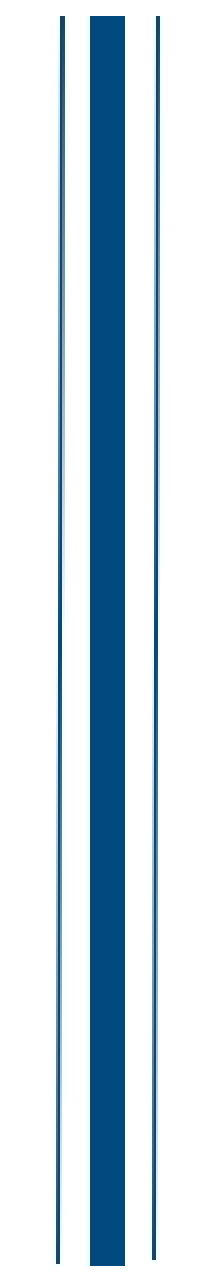
\includegraphics[width=0.5cm,height=15.3cm]{LineaAzul.eps}}
	    \put(-37,-275){\includegraphics[width=3cm,height=2.5cm]{logoescom.eps}}
	\end{picture}}
	\parbox{14cm}{\vspace{1cm} 
	\begin{center}
	    {\fontsize{20}{30}\textbf{ INSTITUTO POLITÉCNICO NACIONAL}}\\[0.2cm]
	    
	    {\fontsize{16}{20} \textbf{ESCUELA SUPERIOR DE CÓMPUTO}}\vspace{1cm}\\[1cm]
	    {\fontsize{20}{20} \textbf{ESCOM}}\vspace{2cm}\\
	    
	    {\fontsize{14}{20} \textit{Trabajo Terminal}}\vspace{1cm}\\
	    {\fontsize{16}{20} \textbf{``Yolotl: un videojuego para fomentar la cultura''}}\vspace{0.5cm}\\
	    {\fontsize{14}{20} \textit{2017-A035}}\vspace{1.5cm}\\
	    {\fontsize{14}{20} \textit{Presentan}}\\
	    {\fontsize{14}{20} \textbf{Hernández Bautista Yasmine Pilar}}\vspace{1cm}\\
	   	{\fontsize{14}{20} \textbf{Márquez Hernández Karla Rocío}}\vspace{1.5cm}\\
	   \fontsize{14}{20} \textit{Directores}\\

	    
	    
{\fboxrule=0pt \fboxsep=6pt	    
\fbox{{\fontsize{14}{20} \textbf{\textit{M. en C. Rafael Norman Saucedo Delgado}}.}\vspace{3.5cm}}
\fbox{{\fontsize{14}{20} \textbf{\textit{Lic. Ulises Vélez Saldaña}}.}\vspace{3.5cm}}}\\[3.5cm]
\end{center}
	    
	    \hfill  \fontsize{12}{20} \textit{Noviembre 2017}
	    
	}
\end{titlepage}

\thispagestyle{empty}

\parbox{18cm}{
\parbox{1.5cm}{
\includegraphics[width=1.5cm,height=2.5cm]{IPN.eps}
}
\parbox{12cm}{
\centering{{\fontsize{16}{0}\textbf{ INSTITUTO POLITÉCNICO NACIONAL}}\\	
{\fontsize{16}{0} \textbf{ESCUELA SUPERIOR DE CÓMPUTO}}}
}
\parbox{1.5cm}{
\includegraphics[width=2.5cm,height=2cm]{logoescom.eps}
}\vspace{1.5cm} 
}

	\begin{center}
	    
	    
\begin{multicols}{2} 
\raggedright{{\fontsize{14}{20} No. de TT:2017-A035}} 

\raggedleft{{\fontsize{14}{20} 17 de noviembre de 2017}}
\end{multicols}\vspace{1cm}

	    {\fontsize{14}{20} \textit{Documento Técnico Parte A}}\vspace{1cm}\\
	    {\fontsize{16}{20} \textbf{``Yolotl: un videojuego para fomentar la cultura''}}\vspace{1.5cm}\\
	    {\fontsize{14}{20} \textit{Presentan}}\\
	    {\fontsize{14}{20} \textbf{Hernández Baustista Yasmine Pilar\footnote{daughterofthewind10@gmail.com}}}\vspace{1cm}\\
	    {\fontsize{14}{20} \textbf{Márquez Hernández Karla Rocío\footnote{yolotl.escom@gmail.com}}}\vspace{1cm}\\
	   
	   \fontsize{14}{20} \textit{Directores}\vspace{1.5cm}\\
	    
	    
{\fboxrule=0pt \fboxsep=12pt	    
\fbox{{\fontsize{14}{20} \textbf{\textit{M. en C. Rafael Norman Saucedo Delgado}}.}\vspace{5.5cm}}
\fbox{{\fontsize{14}{20} \textbf{\textit{Lic. Ulises V\'elez Saldaña}}.}
}}
\end{center}
\begin{center}
{\fontsize{14}{20} \textbf{RESUMEN}}
\end{center}
En México la industria de videojuegos tiene una alta demanda de consumo; sin embargo, existen pocos estudios que desarrollen videojuegos basados en la cultura mexicana. Actualmente en México existe un fuerte desinterés en la cultura nacional. El presente trabajo terminal consiste en el desarrollo de un videojuego que fomente la cultura con temática de la cultura mexica. 
\\
 
\textbf{\textit{Palabras clave}}. –  Cultura mexica, desarrollo tecnológico, ingeniería de software, videojuego.
	
	\chapter{Advertencia}

%\fcolorbox{red}{white}{
``Este documento contiene información desarrollada por la Escuela Superior de Cómputo del Instituto Politécnico Nacional, a partir de datos y documentos con derecho de propiedad y por lo tanto, su uso quedará restringido a las aplicaciones que explícitamente se convengan.”  La aplicación no convenida exime a la escuela su responsabilidad técnica y da lugar a las consecuencias legales que para tal efecto se determinen. Información adicional sobre este reporte técnico podrá obtenerse en: La Subdirección Académica de la Escuela Superior de Cómputo del Instituto Politécnico Nacional, situada en Av. Juan de Dios Bátiz s/n Teléfono: 57296000, extensión 52000.
%}

	
	
	\tableofcontents
	
	\mainmatter
	\chapter{Introducción}
	\chapter{Planteamiento del problema} 
	\section{Contexto}
En México existe un problema de deficiencia en el sistema educativo, así lo
señalan diferentes pruebas cuya finalidad son medir y comparar el nivel de 
conocimientos de los estudiantes mexicanos entre entidades estatales dentro del 
territorio nacional y con respecto a otros países. El Programa para la Evaluación
 Internacional de Estudiantes (P.I.S.A.) es una de las pruebas encargadas de 
medir el desempeño del sistema educativo de un país. Esta prueba es realizada por 
la Organización para la Cooperación y el Desarrollo Económico (O.C.D.E.). La O.C.D.E 
esta compuesta por 35 países, entre ellos México. La prueba P.I.S.A. tiene como 
objetivo evaluar hasta que punto los estudiantes cercanos a concluir la educación 
obligatoria han desarrollado los conocimientos y habilidades necesarios para la 
participación plena en la sociedad del saber\cite{RefOCDE}, por lo que se realiza en 
jóvenes de 15 años en 72 países. En el 2016, México ocupó lugares 58, 55 y 56 de
 en la prueba PISA en materia de conocimiento científico, lectura y comprensión 
lectora y matemáticas respectivamente\cite{RefPisa}, lo que ubica el nivel de 
aprendizaje en México por debajo de la media internacional.
        \\
        \par
Anudado a las deficiencias del sistema educativo, México presenta un 
déficit en cuanto a libros libros leídos, esto se puede decir con base 
en diferentes estudios que determinaron la cantidad de libros leídos en 
México, de los cuales tres son los más citados por especialistas en el 
tema, éstos son: 
	\begin{itemize}
		\item El realizado por la Organización de las Naciones Unidas (O.N.U.), en 
		donde México tuvo una media de 2.8 libros leídos anualmente, ubicando a México
		 en el penúltimo lugar de entre 108 países\cite{RefLibrosCantidad}.
        \item  La Encuesta Nacional de Lectura y Escritura de Conaculta 
        en donde se obtuvo un promedio 5.3 libros al año, entre mexicanos 
        mayores a 13 años\cite{RefLibrosCantidad}.
        \item El más reciente Modulo de Lecutura (M.O.L.E.C.) del Instituto Nacional 
        de Estadística y Geografía(I.N.E.G.I.). Con base en los resultados obtenidos 
        durante la encuesta del 2018, el 76.4\% de la población mayor de 18 años
         alfabeta lee algún material considerado por el M.O.L.E.C; esta cifra 
         presupone una disminución del 3.3\% con respecto al 2017. De este 76.4\% 
         solo el 45.1\% tiene como material de lectura los libros, de los cuales 
         el 40.8\% prefiere los libros de literatura\cite{RefModuloLectura}.
	\end{itemize}	    


	\chapter{Marco teórico conceptual}
	\section{Videojuego.}\label{Videojuego}
	En esta sección se define lo que es un videojuego, sus características, los tipos de 
	clasificaciones, haciendo principal inacpie en las dos de las más importantes: la
	 clasificación por su contenido y por su jugabilidad, finalizando con la el 
	 estado de la industria del videojuego a nivel internacional y en México.
	
	\subsection{¿Qué es un videojuego?}\label{Defvideojuego}
El grupo Carricay define al videojuego como: "una aplicación interactiva orientada
 al entretenimiento que, a través de ciertos mandos o controles, permite simular 
 experiencias en la pantalla de un televisor, una computadora u otro dispositivo 
 electrónico"\cite{Ref_DefVideo}.
	
	\subsection{Caracteristicas del videojuego.}\label{CaracVideojuego}
	Al igual que con otros productos tecnológicos, la evolución de los videojuegos 
	ha sido vertiginosa, resultando complicado mencionar características comunes 
	para todos los videojuegos. Sin embargo, en el libro “Marketing y videojuegos: 
	Product pacement, in-game, adevertising y advergaming” se menciona que existen seis 
	características comunes en los videojuegos: Interactividad, entretenimiento, 
	jugabilidad, simulación \textbackslash virtualidad, inmersión y multiplataformidad 
	\cite{RefCarac}; a continuación se hace menciona en que consisten cinco de las seis 
	características, esto debido a que la última no se encuentra presente en todos los 
	juegos y el mismo autor de la obra la menciona como una caracteristica opcional a 
	tomar en cuenta:
	%%para los autores mejor mencionar obra
	\begin{itemize}
		\item \textbf{Interactividad:} En el articulo "Defining Virtual Reality:
		 Dimensions Determining Telepresence" se define la interactividad como la 
		 capacidad de los usuarios para participar y modificar la forma y el contenido 
		 de un entorno mediado en tiempo real\cite{RefInteractividad}.  
		
		\item \textbf{Entretenimiento:} en el articulo "Las Tecnologías del
		 Entretenimiento: Pasado, Presente y Futuro", el entretenimiento "se asocia, 
		 usualmente, de hacer algo que nos divierte, algo que podemos hacer solos o con 
		 otros, para entretenernos o divertirnos, en nuestro tiempo libre, o tal vez, 
		 algo que nos relaje o que nos haga reír"\cite{RefEntretenimiento}. 
		
		\item \textbf{Jugabilidad:} en el libro “Marketing y videojuegos: 
	Product pacement, in-game, adevertising y advergaming” se define la jugabilidad 
	como "la relación que existe entre todas las acciones reacciones e interacciones
	 tanto del videojugador como el videojuego como entre los propios sistemas y 
	 subsistemas programados en el videojuego"\cite{RefCarac}.
		
		\item \textbf{Simulación \textbackslash Virtualidad:} La simulación "se trata 
		de una representación a medida cuyo objetivo nos permite interactuar y 
		relacionarnos con lo representado según nuestros intereses"\cite{RefCarac}.
		
		\item \textbf{Inmersión:} Con base en el libro "La vida en la pantalla: La
		 construcción de la identidad en la era de internet", la inmersión es un 
		 proceso psicológico que se produce cuando la persona deja de percibir de 
		 forma clara su medio natural al concentrar toda su atención en un objeto,
		  narración, imagen o idea que le sumerge en un medio artificial 
		  \cite{RefInmersion}. Por su parte en la tesis "Libertad dirigida: Análisis 
		  formal del videojuego como sistema, su estructura y su avataridad", la 
		  inmersión se entiende como la coherencia de la ficción del juego y su 
		  aceptación por el jugador.\cite{refInmersionNavarro}  
	\end{itemize}
		
	\subsection{Clasificación del vidoejuego.}\label{ClasiVideojuego}
	Los videojuegos pueden ser clasificados con base a diferentes factores según lo que 
	se desee saber de ellos. Las clasificaciones más populares son basándose en:
        \begin{itemize}     
                \item \textbf{Contenido:} Esta clasificación evaluá desde la temática
                 del videojuego, dificultad, el argumento(en caso de que el videojuego 
                 tenga), etc. y agrupa los juegos determinando el publico para el que 
                 son aptos.
                \item \textbf{Jugabilidad}: Clasificación se basa en los puntos en común 
                de la jugabilidad entre videojuegos y los clasifica en diferentes 
                géneros; en esta clasificación un videojuego puede estar en dos géneros 
                a la vez.
                \item \textbf{Plataforma}: Clasificación hecha con base en la 
                plataforma para la que el juego se encuentra disponible tales como
                 computadoras, móviles o consolas.
                \item \textbf{Cantidad de jugadores que el juego soporta al mismo
                 tiempo:} Puede se un solo jugador o múltiples jugadores.
                \item \textbf{Conectividad:} Esta clasificación se basa en si 
                el juego necesita de conexión a Internet o no para funcionar o para 
                algunas de sus funcionalidades. 
        \end{itemize}
        En esta sección únicamente se va a profundizar en las clasificaciones por 
        contenido y jugabilidad.      
	
		\subsubsection{Clasificación por contenido.}
			Esta clasificación consiste en evaluar los contenidos y elementos de
			 interactividad de los videojuegos y clasificarlos en los grupos de edad 
			 para los que son aptos \cite{RefESRB}. El objetivo de esta clasificación es 
			 que los consumidores puedan comprar videojuegos de manera informada sobre 
			 el contenido de los juegos.                  
             \\
             \par                    
             La necesidad de clasificar a los juegos por su contenido nació en 1994 
             luego de la controversia que trajo el estreno de Mortal Kombat
             \textregistered, juego de peleas famoso por su alto contenido de violencia 
             \cite{RefClasificacion}; siendo este alto contenido de violencia 
             lo que levantó la preocupación entre diferentes jefes de familia 
             con respecto al tipo de contenido que sus hijos tenían acceso con 
             los videojuegos. Actualmente existen diversas organizaciones 
             se encargan de clasificar a los videojuegos por su contenido. A 
             continuación se mencionan las más importantes:
                        
                        \begin{itemize}
                                \item Organización de clasificación de entretenimiento
                                 informático (CERO, por sus siglas en inglés).
                                \item Autocontrol en el Software de Entretenimiento 
                                (USK, por sus siglas en Aleman).
                                \item Junta de Clasificación de Software de 
                                Entretenimiento (ESRB, por sus siglas en inglés).
                                \item Información paneuropea del juego (PEGI, por sus 
                                siglas en inglés).
                        \end{itemize}                     
                
        Cada una opera en determinada zona geográfica, esto debido a las diferencias
         culturales entre países. En algunos países, las instituciones 
         gubernamentales son las encargadas de la clasificación de los 
         videojuegos, tal es el caso de China y Rusia. Si bien no existe ninguna 
         normatización internacional que obligue a los creadores de videojuegos 
         a someter sus productos a esta evaluación(salvo por algunos países con 
         este tipo de legislaciones), algunas distribuidoras como Nintendo
         \textregistered, Sony\textregistered, Microsoft\textregistered marcan 
         como una condición obligatoria para todos aquellos que deseen publicar 
         contenido en sus dispositivos \cite{RefObligacion}.
        \\
        \par
        Actualmente México esta afiliado a la ERSB, por lo que en la siguiente 
        sección se profundiza en ésta; sin embargo, es importante mencionar que 
        se desconoce si seguirá bajo este estándar ya que en el 2017, el Senado 
        mexicano aprobó una nueva legislación en materia de clasificación de 
        contenido de videojuegos \cite{RefRegulacionMex}. 

	\subsubsection{Junta de Clasificación de Software de Entretenimiento.}
	La ERSB fue fundada en 1994; su centro de operaciones se ubica en Estados 
	Unidos y Canadá. Actualmente cuenta opera en Norteamérica y América latina.
        \\
        \par
	Los juegos que han sido clasificados por la ERSB cuentan con la etiqueta (ver 
	figura \ref{fig_etiquetaERSB}) en su empaque tal como se muestra en la figura
	 \ref{fig_caratulaERSB}. 
        \\
        \par
        La etiqueta que emite la ERSB esta compuesta por tres partes:
                \begin{itemize}
                        \item \textbf{Categoría de clasificación:} Sugiere la edad
                         adecuada para el público del videojuego, ver figura 
                         \ref{fig_etiquetaERSB}.
                        \item \textbf{Descriptores de contenido:} Indica los elementos
                         que motivaron la Categoría de clasificación o son motivo de 
                         preocupación para el consumidor.
                        \item \textbf{Elementos interactivos:} Informan acerca de los 
                        aspectos interactivos de los productos, como recursos de memoria 						necesarios para su funcionamiento, uso de conexión a internet o 							cantidad de jugadores de manera simultanea.
                \end{itemize}      	
	
		\begin{figure}
					\centering
					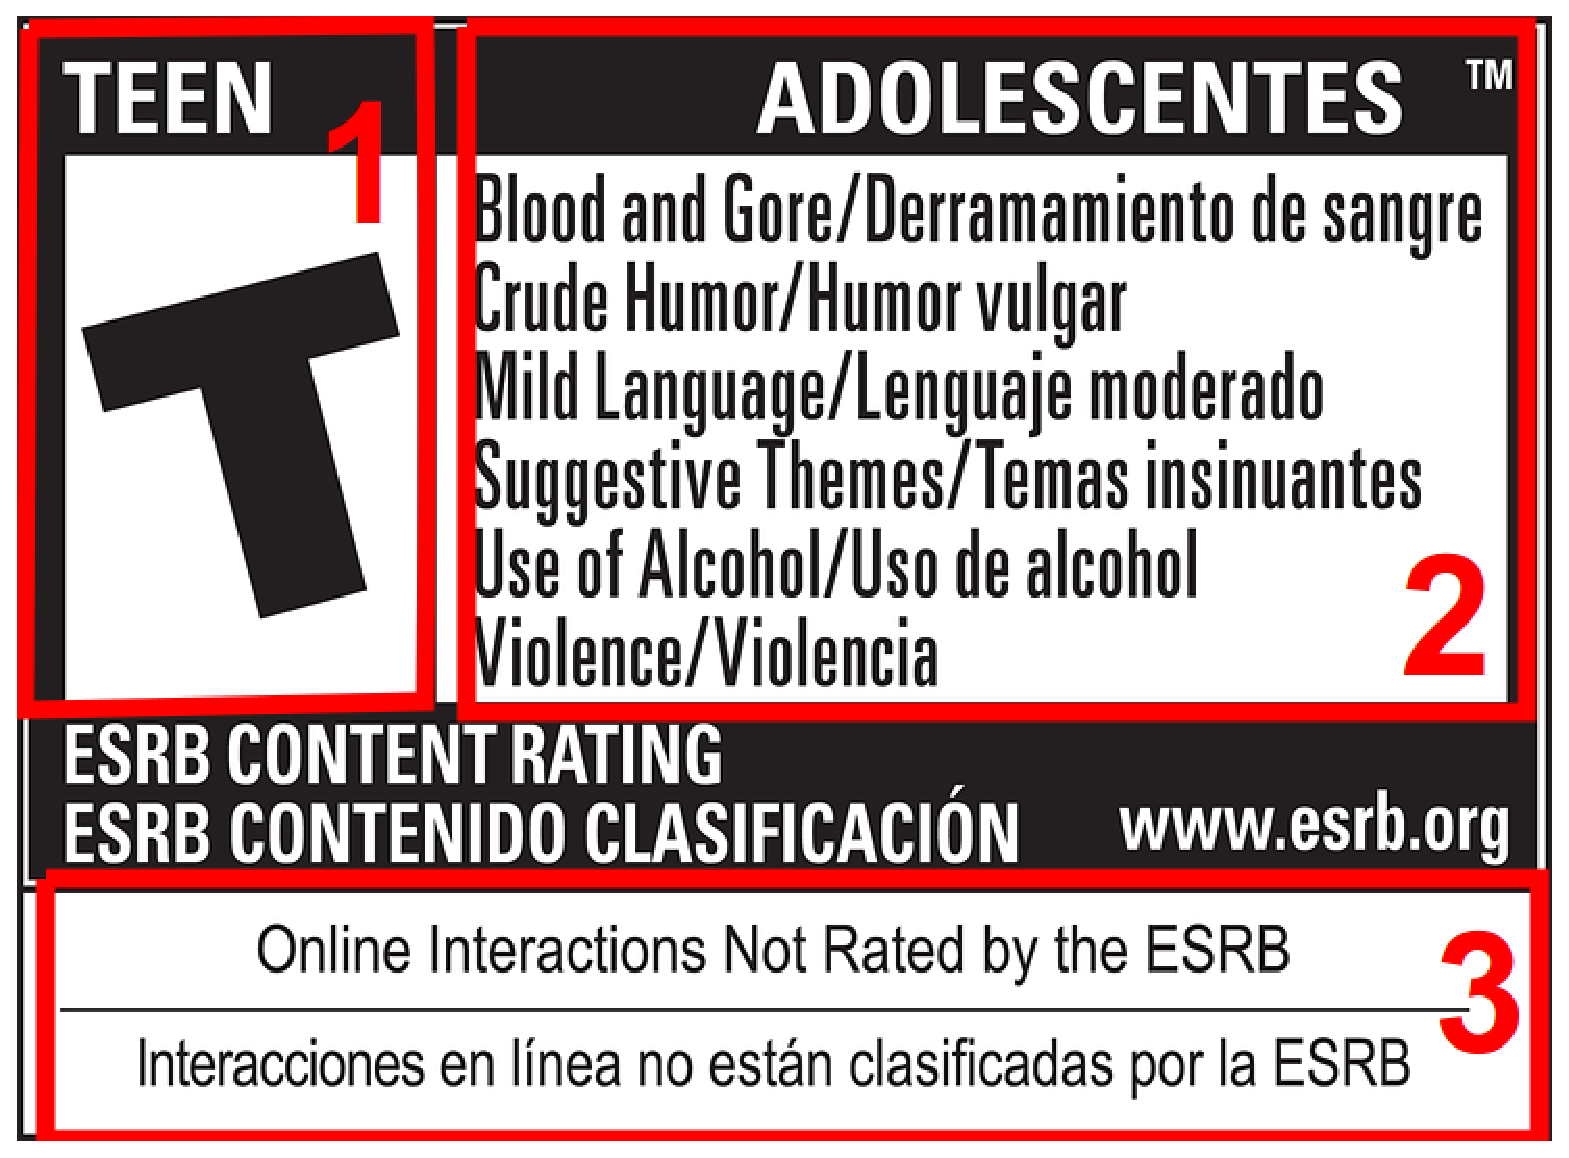
\includegraphics[width=0.4 \textwidth]{03MarcoTeoricoA/imagenes/etiqueta.eps}
					\caption{Etiqueta de clasificación de la ERSB. Esta compuesta de 
					tres partes: 1. Categorías de clasificación. 2. Descriptores de 
					contenido. 3. Elementos Interactivos $ [Imagen] (s/f)$ Recuperado 
					de: \url{http://media.blizzard.com/global-video-player/ratings-png/wow-cataclysm-esrb-esmx.png} } 
					\label{fig_etiquetaERSB}
		\end{figure}
		%,natwidth=737,natheight=540  ,natwidth=407,natheight=608
		\begin{figure}
					\centering
					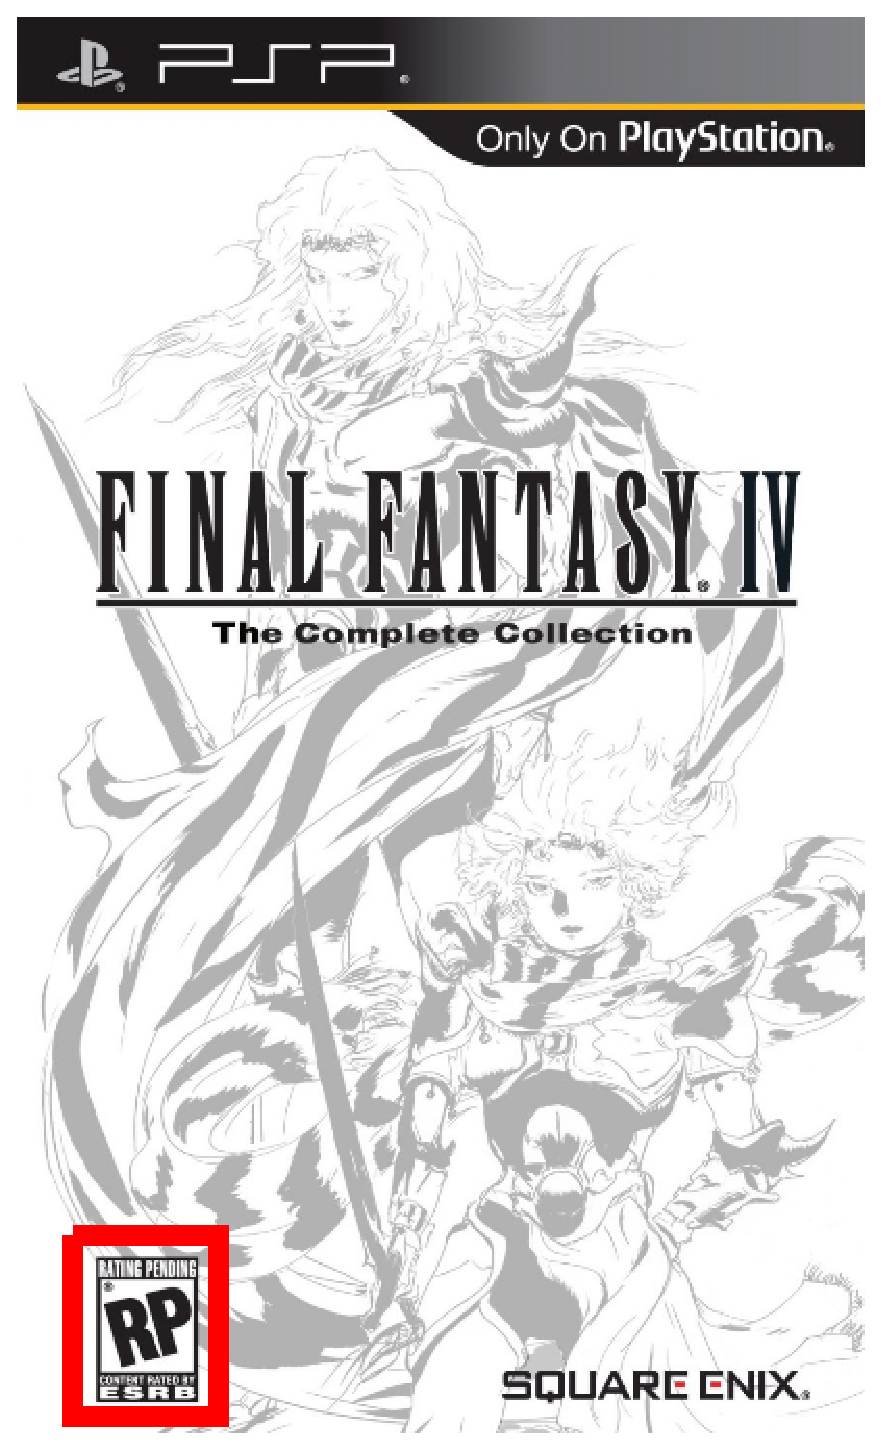
\includegraphics[width=0.3 \textwidth]{03MarcoTeoricoA/imagenes/FFCaratula.eps}
					\caption{Carátula de un juego con la etiqueta de clasificación ESRB 
					$[Imagen] (s/f)$ Recuperado de: \url{https://
					vignette.wikia.nocookie.net/es.finalfantasy/images/1/1c/
					FF4PSP\_NA\_Caratula.PNG/revision/latest?cb=20110301012441} } 
					\label{fig_caratulaERSB}
		\end{figure}
		\subsubsection{Clasificación por jugabilidad.}
		Esta clasificación es empleada por la industria para diferenciar los tipos de 
		juegos y de jugadores. A continuación se presenta la clasificación propuesta 
		en el libro "Juego. Historia, Teoría y Práctica del Diseño Conceptual de 
		Videojuegos"\cite{Ref_JuegoDisenio}  
			\begin{itemize}
			%===== Juegos de accion =====%
				\item \textbf{Juegos de acción:} Son juegos usualmente de temática 
				violenta. El jugador lucha por su supervivencia, para ello se vale 
				de armas o habilidades de  combate. Los juegos de acción se subdividen 
				en:
				\begin{itemize}
					\item \textbf{Juegos de lucha:} Este tipo de juego involucra lucha
					 cuerpo a cuerpo, con una fuerte infliuencia de las artes marciales.
					\item \textbf{Juegos de disparos:} Son aquellos en donde el jugador 
					mueve a su personaje para superar diversos escenarios en donde el 
					jugador debe de hacer uso de su armamento para lograr completar el 
					nivel.
					\item \textbf{Juego de plataformas:} El jugador debe de controlar a 
					un personaje con el que se dezplazará saltando entre plataformas y 
					esquivando todo tipo de obstáculos y enemigos.
				\end{itemize}
			%==== Juegos de estrategia ====%
				\item \textbf{Juegos de estrategia:} Para que el jugador logre sus 
				objetivos en este tipo de juegos, éste debe de planear una estrategia, 
				normalmente a lago plazo. La temática del juego de estrategia se 
				relaciona más con la escala y la visión. Lo juegos de estrategia 
				usualmente involucran mapas de gran tamaño, visión sobre el campo, 
				gestión de recursos, manejo de tropas, desarrollo de recursos, comercio 
				e intercambio de recursos, modificadores del campo, control de 
				territorio, etc.
			%==== Juegos de Rol ====%
				\item \textbf{Juegos de Rol:} Estos juegos tienen sus orígenes en los 
				juegos de rol de mesa. La mecánica de los juegos de rol gira en torno a 
				un grupo de héroes, con habilidades y progresión definidos; el grupo de 
				héroes debe de trabajar coordinadamente para cumplir un objetivo; estos 
				héroes pueden ser controlados por un solo jugador o por varios. El 
				jugador deberá explorar un mundo de gran tamaño haciendo evolucionar a 
				sus personajes y sus habilidades. En los juegos de rol, el uso y 
				recolección de objetos tiene un gran peso en la capacidad de avance del 
				jugador.
				\item \textbf{Videojuego de aventura:} Son parecidos a los juegos de 
				Rol; con la peculiaridad de que tienen una progresión más lineal y no 
				se hace tanto énfasis en los combates, siendo su eje principal la 
				narrativa.
				\item \textbf{Videojuegos de deportes:} Son todos aquellos videojuegos 
				que tratan sobre deportes que no involucren la conducción de un 
				vehículo. Pueden ser juegos sobre fútbol, fútbol americano, tenis, etc.
				\item \textbf{Videojuegos de carreras de vehículos:} Son todos aquellos 
				se centran en las carreras con todo tipo de vehículos, mayoritariamente 
				automóviles.
				\item \textbf{Videojuegos {\it puzzle:}} Este tipo de juego involucra 
				la resolución de un problema a partir de la utilización de una serie 
				limitada de recursos, por lo que si los recursos no se utilizan de la 
				manera correcta el problema no podrá ser solucionado.  
			\end{itemize}
			
	\subsection{Industria del videojuego.}\label{IndusVideo}
	El videojuego como producto para masas nace en 1972 con el videojuego de Pong 
	desarrollado por la empresa Atari, es así como nace las primeras maquinas 
	recreativas, ver figura \ref{fig_MaquinaAtari}. En sus inicios los videojuegos se caracterizaban por el uso de 
	pantallas estáticas, entornos bidimensionales y formas abstractas de juego
	\cite{perez2010analisis}. A la aparición de las maquinas recreativas le seguirían 
	las primeras consolas de mesa desarrolladas principalmente por Atari. 
	\\
	\par

	\begin{figure}
					\centering
					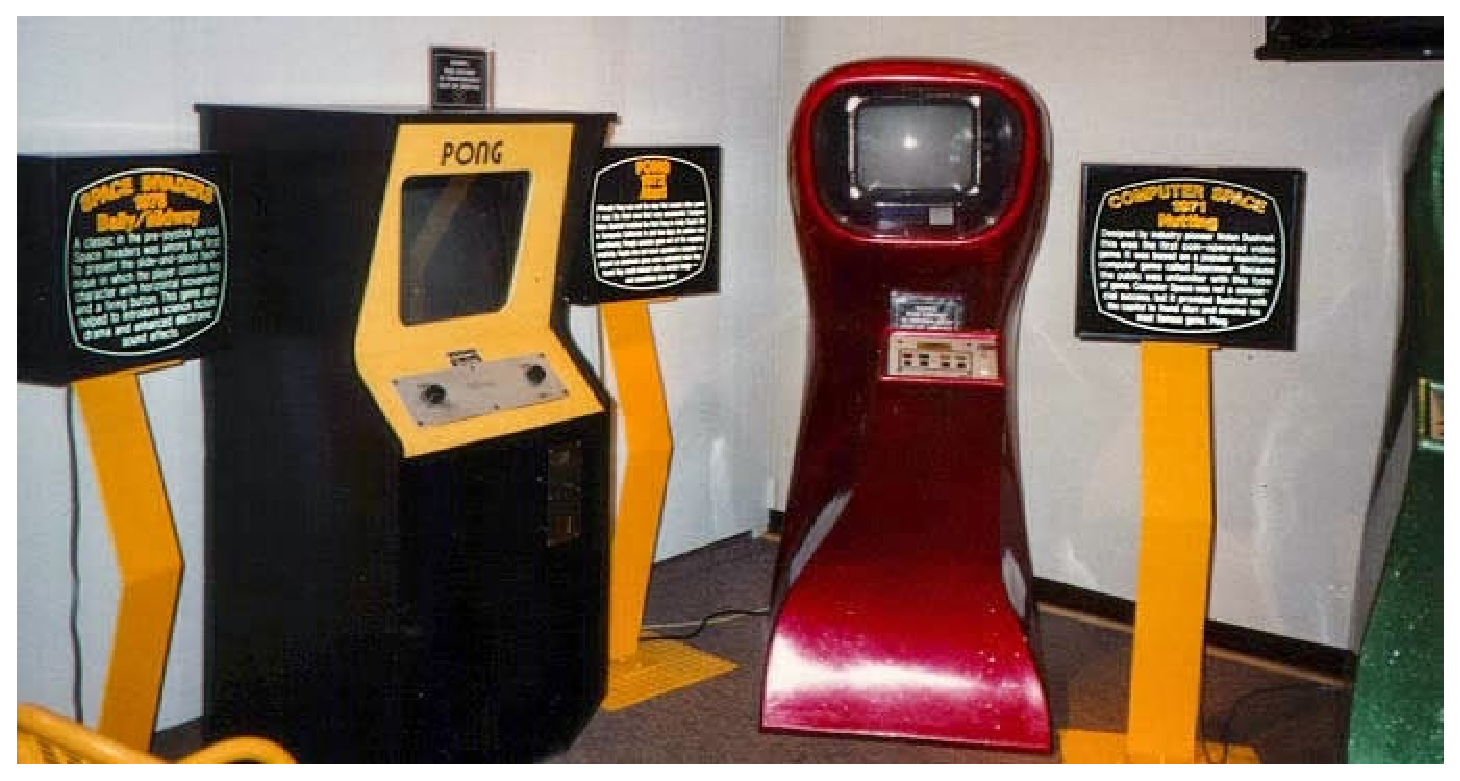
\includegraphics[width=0.5 \textwidth]{03MarcoTeoricoA/imagenes/atari.eps}
					\caption{Primeras maquinas recreativas desarrolladas por Atari 
					$[Imagen] (s/f)$ Recuperado de: \url{http://2.bp.blogspot.com/--98a06VymhA/VKJv2AQbNGI/AAAAAAAAAXU/rASZPNmBMrg/s1600/first\%2Barcades.jpg} } 
					\label{fig_MaquinaAtari}
		\end{figure}	
	
	Durante los años subsecuentes la industria del vidoejuego gozaría de una alta 
	tasa de recuperación; sin embargo la industria entraría en declive 1983, 
	empezando el periodo conocido como la crisis de los videojuegos, misma que 
	afectaría principalmente a las empresas estadounidenses y canadienses. Este 
	periodo duraría hasta 1985 y provocaría una polarización del mercado en donde 
	la industria japonesa de los videojuegos tomaría la ventaja frente a la 
	estadunidense. En 1983 la compañía Nintendo lanza al mercado su primera consola, 
	la Fumicom o Nintendo Entertainment System(NES) como fue conocida en el resto 
	del mundo \cite{belli2008breve}. Nintendo dio inicio a una nueva era para la 
	industria del videojuego con el lanzamiento de títulos que se consagraron como 
	clásicos de la industria y que al día de hoy aun se encuentran vigentes en el 
	mercado tales como Super Mario Bros, The Legend of Zelda, Pokemón, etc (ver figura \ref{fig:Nintendo}).
	\\	
	\par
	
	\begin{figure}
  		\centering
   		\subfigure[Super Mario Bros.] {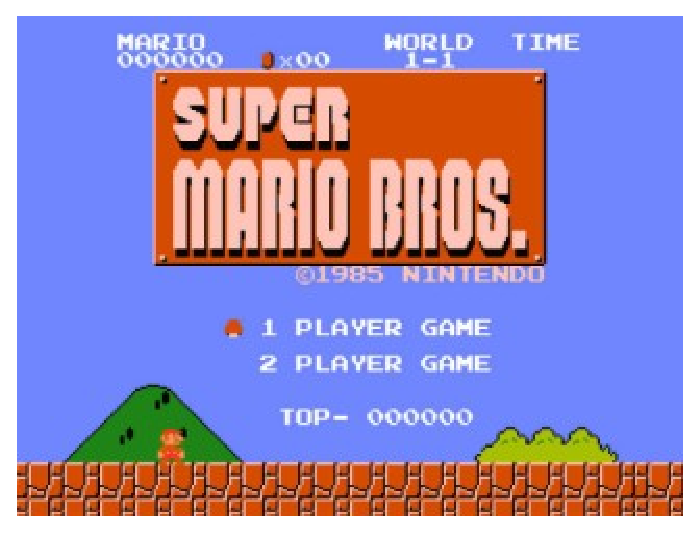
\includegraphics[width=0.3 				\textwidth]{03MarcoTeoricoA/imagenes/mario1.eps}}
   
 		\subfigure[The Legend of Zelda.]{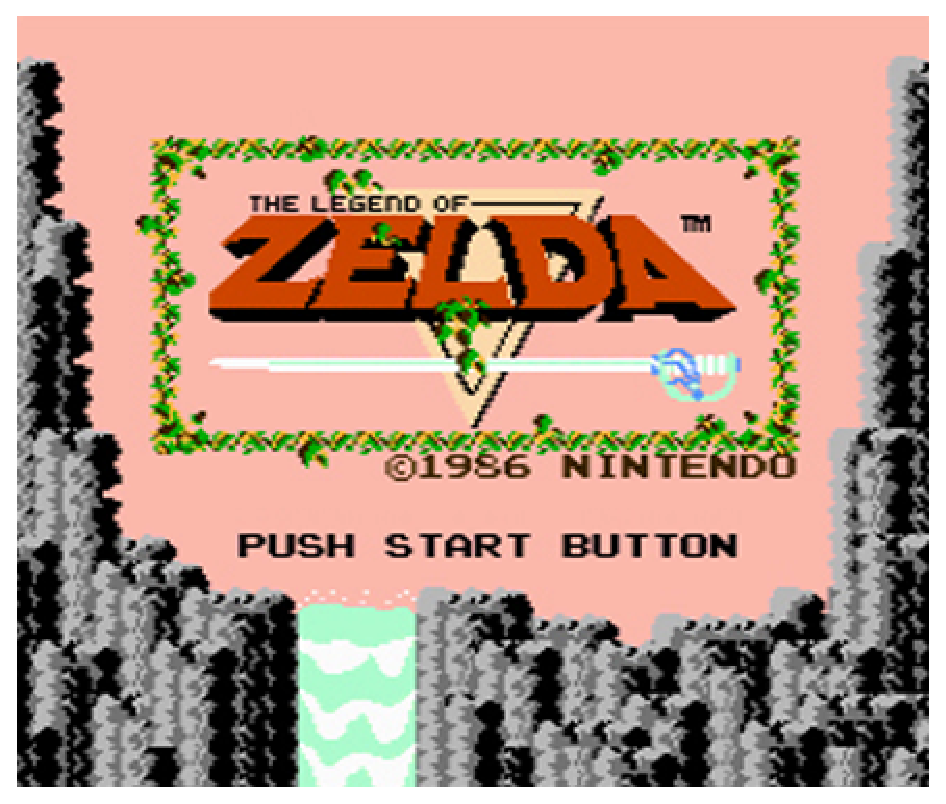
\includegraphics[width=0.3 \textwidth]{03MarcoTeoricoA/imagenes/zelda.eps}}
 	
		\subfigure[Pokemón.] {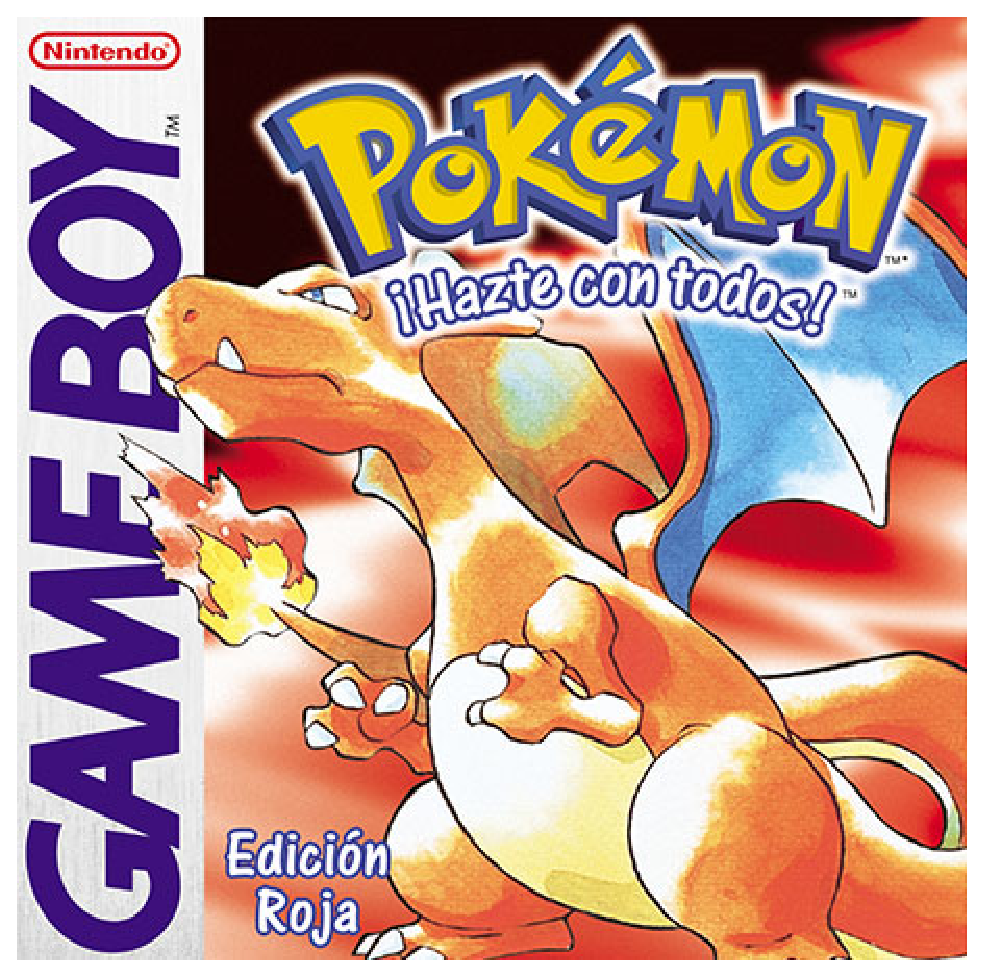
\includegraphics[width=0.3 \textwidth]{03MarcoTeoricoA/imagenes/pokemon.eps}}
  		\caption{Super Mario Bros, The Legend of Zelda y Pokemón son algunas de la franquicias más importantes de la compañía japonesa Nintendo.[Imagen] (s/f) Recuperado de (respectivamente): \url{http://contenidos.enter.co/custom/uploads/2015/09/mario1.jpg}, \url{https://www.hiddentriforce.com/wp-content/uploads/2015/02/10106454_5124592_lz.jpg}, \url{https://vignette.wikia.nocookie.net/es.pokemon/images/d/db/Car\%C3\%A1tula_de_Pok\%C3\%A9mon_Rojo.jpg}}
  		\label{fig:Nintendo}
	\end{figure} 

En las décadas posteriores, la industria del vidoejuego creció a un ritmo 
vertiginoso; no solo se diversifico el mercado con el nacimiento de nuevos 
géneros de videojuegos sino también las innovaciones tecnológicas de hardware 
permitieron crear cada vez mejores experiencias de juegos \cite{belli2008breve}. 
En menos de 20 años los videojuegos pasaron de entornos en dos dimensiones a 
entornos en tercera dimensión, del formato de almacenamiento en cartuchos al 
uso de CDs.	
	
Anualmente la induatria de los videojuegos genera miles de millones de dolares en ganancias, tan solo en el 2017 la industria generó 108.9 mil millones de dolares\cite{Ref_JuegosGanancia}. Estas ganancia fueron generadas un 25\% en Norteamerica, el 24\% en Europa, Medio Oriente y Africa, el 4\% en America latina, siendo la zona con mayor ingresos Asia y la zona del pacifico con el 47\% de ganancias generadas. En cuanto a la distribución de las ganacias con base a las plataformas, los telefonos moviles destronan a las consolas al generar el 32\% de las ganancias, mientras que las consolas han generado el 31\% de las ganancias, seguidas por las computadoras con el 23\%\cite{Ref_JuegosGanancia}.
	\\
	\par 
	%=== To do Poner las imagenes de las graficas de la estadistica
	
	\subsection{Industria del juego en México}
		La industria mexicana de videojuegos, al igual que la latinoamericana, es una industria emergente. Las empresas productoras de videojuegos mexicanas 
	\\
	\par
	México cerró el 2017 con un consumo de videojuegos de 1.4 mil millones de dolares, lo que le valio el doceavo puesto en cuanto a consumo de videojuegos a nivel mundial y el primer lugar en America latina. De acuerdo con los reportes de Unidad de Inteligencia Competitiva (CIU, por sus siglas en inglés) del 2016; en México hay 52.7 millones de jugadores, de los cuales el 71\% juega en dispositivos moviles\cite{Ref_IndusMEx}. Desafortunadamente y en contraposicion con estas cifras el consumo de videojuegos en México esta enforcado en juegos de origen extrangero. 
 
	\section{Desarrollo de videojuegos.}\label{DesVideojuego}
En esta sección se describe el proceso de desarrollo del videojuego, hablando 
sobre los pasos que lleva dicho proceso; para después describir las 
metodologías de desarrollo que se emplean, algunas de las metodologías descritas 
en este apartado son originarias del desarrollo de software convencional pero 
son adaptadas al desarrollo de videojuegos por algunos estudios independientes; es 
importante mencionar que muchas de las metodologías de desarrollo de videojuegos 
son propiedad de las empresas que las utilizan y por lo tanto no son de carácter 
público por lo que no pudieron ser incluidas en este trabajo terminal. Para 
finalizar esta sección se hace mención del software empleado en el desarrollo de 
videojuegos, iniciando con el motor de juego, el cual se define y se explica a 
grandes rasgos su arquitectura.

	\subsection{Linea de producción de un videojuego.}\label{Pipelinevideojuego}
	Una linea de producción son los pasos o fases lógicos y secuenciales requeridos 
	para obtener un producto. Los pasos que componen la linea de producción dependen 
	del producto que se va a fabricar y de la empresa fabricante. 
        \\
        \par    
        Existe una discrepancia en cuanto a que elementos tiene la linea de producción 
        de un videojuego, siendo la planteada por la revista ING la más común. Esta 
        linea consiste en tres etapas\cite{Ref_Desarrollo}:
	\begin{itemize}
		\item \textbf{Concepto:} Es la idea que origina a todo el juego a 
                realizar. Esta puede ser una simple oración en la que se mencione el 
                contexto del juego y su temática o bien puede ser un acuerdo de la 
                compañía desarrolladora para hacer una secuela o una precuela de un 
                videojuego ya existente\cite{Ref_Desarrollo}.
	%===============================		
		\item \textbf{Preproducción:} En esta etapa el equipo de producción redacta 
		el documento de diseño del videojuego, define el argumento, los personajes y 
		la jugabilidad. En esta etapa se determinan todas las limitantes técnicas 
		y creativas que va a tener el proyecto\cite{Ref_Desarrollo}.
	%===============================
		\item \textbf{Producción:} En esta etapa se desarrolla el juego: los artistas 
		desarrollan todos los elementos visuales que se van a emplear, los 
		programadores se encargan de implementar la lógica del juego y la jugabilidad 
		establecida en la etapa de preproducción y el equipo de audio se encarga de 
		generar todos los elementos de audio que conlleva el videojuego
		\cite{Ref_Desarrollo}.
	%===============================
		\item \textbf{Postproducción:} En esta etapa el juego se considera casi 
		terminado y es sometido a diferentes pruebas para medir su rendimiento, 
		identificar todo tipo de errores y solucionarlos. También en esta etapa se 
		intensifican las campañas de promoción para el juego\cite{Ref_Desarrollo}.
\end{itemize}	 

	\subsection{Metodologias de desarrollo de videojuegos.}\label{MetodoVideojuego}
	En esta sección se define lo que es una metodología de desarrollo de software, 
	se mencionan tres metodologías de desarrollo de software que emplea la industria 
	de los videojuegos y al final se menciona una metodología propia 
	del desarrollo de videojuegos. 
	
%======================================================			
		 \subsubsection{¿Qué es una metodología de desarrollo de software?}
	Las metodologías de desarrollo de software son un conjunto de procedimientos, 
	técnicas y ayudas a la documentación para el desarrollo de productos software
	\cite{Ref_metodologia}.	En palabras de Gacitúa: "Una Metodología impone un proceso
	 de forma disciplinada sobre el desarrollo de software con el objetivo de hacerlo 
	 más predecible y eficiente. Una metodología define una representación que permite 
	 facilitar la manipulación de modelos, y la comunicación e intercambio de 
	 información entre todas las partes involucradas en la construcción de un 
	 sistema"\cite{Ref_Metod}. 

%======================================================		
			\subsubsection{Metodología en cascada}
La metodología de desarrollo en cascada o también conocida como modelo de vida 
lineal o básico,  fue propuesta por Royce en 1970 y a partir de entonces ha tenido 
diferentes modificaciones. Sigue una progresión lineal por lo que cualquier error 
que no se haya detectado con antelación afectara todas las fases que le sigan 
provocando una redefinición en el proyecto y por ende un aumento en los costos 
de producción del sistema \cite{Ref:CarCascada}.
Esta metodología se divide en las siguientes etapas:
\begin{itemize}
	\item \textbf{Análisis de los requisitos del software}: En esta etapa se recopilan
	 los requisitos del sistema, se centra especialmente en toda aquella información 
	 que pueda resultar de utilidad en la etapa de diseño, tales como tipos de 
	 usuarios del sistema, reglas de negocio de la empresa, procesos, etc. En esta 
	 etapa se responde la pregunta de ¿Qué se hará? 
	\item \textbf{Diseño}: Esta etapa se caracteriza por definir todas aquellas 
	características que le darán identidad al sistema, tales como la interfaz 
	gráfica, la base de datos, etc. Las características anteriormente definidas 
	se obtendrán de la etapa de análisis. En esta etapa se respondería la pregunta 
	de ¿Cómo se hará? 
	\item \textbf{Codificación}: Terminada la etapa de diseño, lo siguiente es 
	programar y crear todos los elementos necesarios para el funcionamiento del sistema. 
	\item \textbf{Prueba}: Finalizada la decodificación se debe de probar la calidad 
	del sistema. En este punto es importante resaltar que la pruebas no solo abarcan 
	que se confirme que el sistema funcione, sino que también verifica que los 
	usuarios puedan aprender a utilizarlo con facilidad, a su vez tambien se debe de 
	verificar la seguridad de la información y los tiempos de respuesta del sistema.
	\item \textbf{Mantenimiento}: En esta última etapa se realizarán modificaciones 
	al sistema, sin que esto necesariamente signifique que estos cambios se deban 
	a errores de programación, puesto que esta etapa también abarca agregar nueva
	 funcionalidad al sistema o, en caso de que trabaje con protocolos de estándar 
	 internacional, actualizar dichos protocolos \cite{Ref:CarCascada}. 
\end{itemize}
Algunos de los inconvenientes que presenta son:
\begin{itemize}
	\item No refleja el proceso de desarrollo real.
	\item Tiempos largos de desarrollo.
	\item Poca comunicación con el cliente.
	\item Revisiones de proyecto de gran complejidad.
\end{itemize}

%================================================
	\subsubsection{Metodología en Scrum}
Desarrollada por Ikujiro Nonaka e Hirotaka Takeuchi a principios de los 80’s, 
esta metodología le debe su nombre a la formación scrum de los jugadores de ruby. 
Scrum es una metodología eficaz para proyectos con requisitos inestables que 
demandan flexibilidad y rapidez, esto principalmente a su naturaleza iterativa 
e incremental \cite{Ref_DefScrum}.  
\\
\par
Scrum parte de la visión general que se desea que el producto alcance; a partir de 
esta visión se inicia la división del proyecto en diferentes módulos. Scrum 
implementa una jerarquía entre los módulos en donde los módulos de mayor jerarquía 
son los que se desarrollaran al inicio del proyecto o durante las primeras 
iteraciones (sprint). Cada sprint tendrá una duración de hasta seis semanas a lo máximo 
\cite{Ref_ScrumRef}. 
\\
\par
Durante el proceso de desarrollo del sprint, el equipo tendrá reuniones diarias 
en donde se definirán metas diarias para lograr completar el objetivo del sprint. 
Estas reuniones deberán de ser de corta duración (no más de quince minutos) y 
recibirán el nombre de scrum diario. Al final de cada sprint, el equipo contará 
con un módulo funcional que el cliente podrá utilizar sin que el sistema este 
completado.
\\
\par
Cada sprint se compone de las siguientes fases:
\begin{itemize}
	\item \textbf{Concepto}: se define a grandes rasgos las características del 
	producto y se asigna a un equipo para desarrollarlo.
	\item \textbf{Especulación}: Con la información del concepto se delimita el 
	producto, siendo las principales limitantes los tiempos y los costes. Esta es 
	la fase más larga del sprint. En esta etapa se desarrolla basándose en la 
	funcionalidad esperada por el concepto.
	\item \textbf{Exploración}: El producto desarrollado se integra al proyecto.
	\item \textbf{Revisión}: Se revisa lo construido y se contrasta con los objetivos 
	deseados.
	\item \textbf{Cierre}: Se entrega el producto en la fecha programada, esta etapa 
	no siempre significa el fin del proyecto; en ocasiones marca el inicio de la etapa 
	de mantenimiento \cite{Ref_ScrumGuia}. 
\end{itemize}
Uno de los principales componentes de la metodología scrum son los roles, es decir 
el papel que cada integrante del equipo desempeñara durante el proceso de desarrollo.
 Los roles se dividen en dos grupos:
\begin{itemize}
	\item \textbf{Cerdos} : Son los que están comprometidos con el proyecto y el proceso 
	de Scrum.
		\begin{itemize}
			\item \textbf{Product owner}: Es el jefe del proyecto y por lo tanto es 
			quien toma las decisiones. Esta persona es quien conoce más del proyecto y 
			las necesidades del cliente. Es el puente de comunicación entre el 
			cliente y el resto del equipo. 
			\item \textbf{Scrum Master}: Se encarga de monitorear que la metodología y 
			el modelo funcionen. Es quien toma las decisiones necesarias para 
			eliminar cualquier inconveniente que pueda surgir durante el proceso 
			de desarrollo. 
			\item \textbf{Equipo de desarrollo}: Estas personas reciben el objetivo a 
			cumplir del Product owner y cuentan con la capacidad de tomar las decisiones 
			necesarias para alcanzar dicho objetivo.
		\end{itemize}
	\item \textbf{Gallinas}: Personas que no participan de manera directa en el 
	desarrollo, sin embargo, su retroalimentación da pie a la planeación de los sprints.
		\begin{itemize}
			\item \textbf{Usuarios}: Son quienes utilizaran el producto.
			\item \textbf{Stakeholders}: Son quienes el proyecto les aportara algún 
			beneficio. Participan en las revisiones del sprint.
			\item \textbf{Manager}: Toma las decisiones finales. Participa en la 
			selección de objetivos y en la toma de requerimientos\cite{Ref_ScrumRef}.
		\end{itemize}
\end{itemize}

%=============================
\subsubsection{Metodología de Programación extrema}
La metodología de programación extrema o metodología XP(por sus siglas en inglés) fue
 desarrollada por Kent Beck en 1999 basándose en la simplicidad, la comunicación 
 y le retroalimentación de código. Es una metodología de desarrollo ágil y 
 adaptable, soporta cambios de requerimientos sobre la marcha. Su principal 
 objetivo es aumentar la productividad y minimizar los procesos burocráticos, 
 por lo que el software funcional tiene mayor importancia que la documentación
 \cite{Ref_XP}.
\\
\par
  XP se fundamenta en doce principios que se agrupan en cuatro categorías. A 
  continuación, se hará mención de estos principios:
\begin{itemize}
	\item \textbf{Retroalimentación}:
		\begin{itemize}
			\item \textbf{Principio de pruebas}: Se define la el periodo de pruebas de 
			funcionalidad del software a partir de sus entradas y salidas como si se 
			tratara de una caja negra.
			\item \textbf{Planificación}: El cliente o su representante definirá sus 
			necesidades y sobre ellas se redactará un documento, el cual servirá para 
			establecer los tiempos de entregas y de pruebas del producto.
			\item \textbf{Cliente in-situ}: El cliente o su representante se integrarán 
			al equipo de trabajo con la finalidad de que participen en la planeación de 
			tareas y en la definición de la funcionalidad del sistema. Esta estrategia 
			se implementa para minimizar los tiempos de inactividad entre reuniones y 
			 disminuye la documentación a redactar.
			\item \textbf{Pair-programming}: Se asignan parejas de programadores para 
			desarrollar el producto. Esto generará mejores resultados en menores costos.
		\end{itemize}
	\item \textbf{Proceso continuo en lugar de por bloques.}
		\begin{itemize}
			\item \textbf{Integración continua}: Se implementan progresivamente las 
			nuevas características del software. Esta integración no se hace de manera 
			modular ni planeada.
			\item \textbf{Refactorización}: La eliminación de código duplicado o 
			ineficiente les permite a los programadores mejorar sus propuestas en cada 
			entregable.
			\item \textbf{Entregas pequeñas}: Los tiempos de entregas son cortos y 
			permiten la evaluación del sistema bajo escenarios reales.
		\end{itemize}
	\item \textbf{Entendimiento compartido}.
		\begin{itemize}
			\item \textbf{Diseño simple}: El programa que se utiliza en los entregables 
			es aquel que tenga la mayor simplicidad y cubra las necesidades del cliente.
			\item \textbf{Metáfora}: expresa la visión evolutiva del proyecto y define 
			los objetivos del sistema mediante una historia.
			\item \textbf{Propiedad colectiva del código}: Todos los programadores son 
			dueños del programa y de las responsabilidades del programa. Un programa con 
			muchos programadores trabajando en él es menos propenso a errores. 
			\item \textbf{Estándar de programación}: Se define la estructura que tendrá 
			el programa a la hora de ser escrito, esto para dar la impresión de que una 
			sola persona trabajo en él.
		\end{itemize}
	\item \textbf{Bienestar del programador.}
		\begin{itemize}
			\item \textbf{Semana de 40 horas}: Se minimizan las jornadas de trabajo 
			excesivas para grantizar el mejor desempeño del equipo
			\cite{Ref_XPPrincipios}.
		\end{itemize}
\end{itemize}
Tal como se puede observar XP, es una metodología fuertemente orientada hacia los 
miembros del equipo, su bienestar, la interacción entre ellos y en su aprendizaje.

%==========================================
\subsubsection{Metodología Huddle}
Huddle es una metodología creada por el Instituto de Ingeniería y Tecnología de
 Universidad Autónoma de Ciudad Juárez. Huddle recibe su nombre por las reuniones 
 que se realizan en el futbol americano antes de cada jugada. Su funcionalidad 
 se basa en la metodología Scrum, con la diferencia de que está orientada al
  desarrollo de videojuegos.  De naturaleza ágil, resulta óptimo para equipos 
  multidisciplinarios de 5 a 10 personas; es iterativa, incremental y evolutiva 
  \cite{Ref_Huddle}.
\\
\par
Huddle se divide en tres etapas: 
	\begin{itemize}
		\item \textbf{Preproducción}: Consiste en la planeación del juego. En esta etapa 
		se redactará el documento de diseño; este documento contendrá la idea 
		general del juego, su escritura deberá de ser tal que todos los miembros 
		del equipo pueden entenderlo y darse una idea de cómo será el juego una vez 
		que se haya terminado. En esta etapa se definirá el argumento del juego, 
		sus personajes, el género del juego, sus mecánicas, la música, los efectos de 
		sonido, los efectos especiales y su funcionalidad. Huddle proporciona 
		plantilla para realizar este documento, dejando la posibilidad de 
		modificarlo según el equipo considere oportuno.
		\item \textbf{Producción}: Es la etapa más larga y de mayor importancia. Su 
		organización se basa totalmente en la organización iterativa e incremental 
		de Scrum; es decir se harán reuniones diarias en donde se discutirán los 
		objetivos de la iteración. Antes de finalizar cada Sprint, el módulo se someterá 
		a diferentes pruebas para garantizar su funcionalidad. Cuando un Sprint 
		finaliza, se realiza una reunión en la que los elementos del quipo discuten las 
		decisiones tomadas y analizan cuales fueron las decisiones y acciones más 
		eficientes para retomarlas y desechar aquellas que atrasen al proyecto. Al 
		finalizar esta etapa el equipo contará con las versiones alfa y beta del juego. 
		\item \textbf{Postmorten}: En esta etapa se discuten todos los puntos positivos 
		y negativos del proyecto. En esta evaluación se redactará un documento que 
		permita a futuros proyectos efectuar planes de acción más efectivos
		\cite{Ref_Huddle}.
	\end{itemize}

\subsubsection{El metodo Cerny} \label{MetodoCerny}
Esta metodología fue desarrollada por Mark Cenry, arquitecto del Play Station 4 
de Sony y desarrollador de juegos como Jak and Daxter y Crash Bandicoot. El 
método Centry es un método para el diseño industrial de videojuegos de plataforma 
y acción. Se basa en dar una fuerte libertad creativa al equipo de desarrolladores 
durante la etapa de preproducción con la finalidad de explorar la viabilidad 
del producto; bajo este enfoque se desarrolla un primer prototipo y si de este 
no se obtiene un producto que pueda resultar entretenido para los jugadores el 
proyecto se descarta y se inicia uno nuevo utilizando lo aprendido en el anterior.
\\
\par
El método Cenry se centra en cuatro conceptos:
 \begin{itemize}
 	\item \textbf{Preproducción vs. Postproducción.} 
La etapa de preproducción es la más importante. Esta etapa es definida como una 
etapa caótica y para solventarla se debe de integrar un equipo con los mejores 
diseñadores, programadores y artistas, estos pasaran a ser los lideres de sus 
equipos en la fase de producción \cite{MetodoCerny}.
 \\
 \par
En la preproducción se desarrolla una serie de prototipos que en la etapa de 
producción seran las pautas a seguir para los niveles finales del juego. Es 
importante entender que en la preproducción no se realiza el juego sino se 
diseñan y pulen las mecánicas del mismo. Lo anterior se logra bajo el enfoque 
de las \textbf{3 C’s}: \textbf{personaje(Character) , camara(camera) y control
(controles de movimiento)}. De igual forma en esta etapa se define: La apariencia 
del juego, que tecnologías se utilizaran durante el desarrollo \cite{MetodoCerny}.
\\
\par
Para que esta etapa tenga un producto exitoso el equipo debe aprovechar las 
oportunidades e ideas que vayan surgiendo sin centrase en las limitaciones 
tecnológicas ni en el contexto del proyecto. 
\\
\par
Al termino de esta fase el equipo tendrá un primer demo del juego con la calidad 
suficiente como para ser publicado y un macro documento de diseño. 
\\
\par
	\item \textbf{“Publishable” First Playable.}
El demo de la etapa de preproducción debe de contar con dos niveles de alta calidad. 
Estos niveles deben de incluir: 
	\begin{itemize}
	\item Todo el comportamiento del personaje jugable
	\item Todo el comportamiento de los enemigos y obstáculos,
	\item La tecnología de base y todas las funcionalidades tanto locales como globales.
	\item La implementación de toda la capa artística.
	\item Las mecánicas totalmente definidas.
	\end{itemize}
	

	 \item \textbf{ Macro vs Micro Design.}
Este concepto hace referencia a la documentación que acompaña al videojuego. 
La documentación se divide en:  
	\begin{itemize}
		\item \textbf{El macro diseño}: Se desarrolla durante la etapa de 
		preproducción. Consta de a lo más cinco paginas, contiene información 
		sobre el personaje, sus movimientos y mecánicas más exóticas, de igual 
		forma contiene información sobre los niveles tales como su tamaño, 
		estructura, progresión y contenido; finalmente este documento cuenta con un 
		gráfico o tabla de resumen sobre sus contenido. En este documento se puede 
		agregar arte conceptual del juego y la historia del mismo. La ventaja del uso 
		del macro diseño es que permite una mejor planeación y seguimiento de las 
		actividades ya que los líderes de los equipos saben totalmente a que punto se 
		desea llegar con el juego.
		\item \textbf{El micro diseño}: Se realiza durante la etapa de producción. Esta 
	documentación sigue la estructura de documentos de diseño más clásicos al incluir: 
	scripts, mapas de niveles, diseño y comportamiento de los enemigo, descripción de 
	los obstáculos, descripción del gameplay especial, etc.
	\end{itemize}
 
	\item \textbf{Gameplay testing:}
	Se deben de realizar pruebas exhaustivas de jugabilidad y desempeño. Las pruebas 
	son de vital importancia ya que estas le dirán al equipo de desarrollo que tan 
	rápido el jugador aprende las mecánicas y se inmeciona en el juego. Sin embargo, 
	el equipo debe de evitar la pruebas de focalización como pedir la opinión de 
	los teasters ya que no aportan nada al juego. En lugar de estas pruebas se deben 
	de realizar las que involucren al teaster en el juego, es decir hacerlo jugar 
	el juego mientras se observa sus reacciones a este, dichas reacciones se deben de 
	cuantificar y analizar los resultados.
 \end{itemize}

El metodo Cerny busca desmentir los mitos del desarrollo de vidoejuegos, a continuación se presentan dichos mitos:
	\begin{itemize}
	\item \textbf{“Se puede planear y planificar un horario para la creación de un 
	juego”}. Cerny plantea que esta idea no es compatible con el desarrollo de un 
	videojuego al crear presiones en el equipo y limitar la creatividad del mismo.
	
	\item \textbf{“Se productivo significa no tirar nada”}. Cenry sostiene que en 
	la etapa de preproducción es valido desechar tantos prototipos como sea posible 
	ya que no son el juego en sí sino peldaños para obtener el juego.

	\item \textbf{“La tecnología de vanguardia es importante por lo que es lo primero 
	que debe de desarrollarse”}. Con base en la experiencia de Cenry, al desarrollar 
	primero la tecnología antes que el diseño del juego es que se esta limitando 
	el potencial del juego al potencial de la tecnología.

	\item \textbf{“La revisión constante del proyecto es esencial para su buena 
	gestión”}. De igual forma Cenry plantea que esta idea contradice la naturaleza 
	caotica de la etapa de preproducción, por lo que es imposible de realizar.

	\item \textbf{“La versión alfa es la primera versión jugable”}. En palabras de 
	Cenry: sin importar que la versión alfa o beta sea la primera versión jugable, 
	esta debe de ser de suficiente calidad como para que se pueda publicar.

	\item \textbf{“Un proyecto cancelado es sinónimo de de una mala planeación o un 
	mal equipo”}. Cenry propone que no necesariamente, si durante la etapa de 
	preproducción el equipo no logra desarrollar un demo de alta calidad significa 
	que el proyecto no es viable y por lo tanto es un buen momento para descartar el 
	proyecto.

	\item \textbf{“Entre más definida este la versión inicial del proyecto mayor 
	probabilidad de éxito o a mayor detalle el documento de diseño, mejor para el 
	proyecto”}. Cenry sostiene que este principio es erróneo ya que emplear un largo 
	periodo de tiempo unicamente en la documentación es una perdida de tiempo. Cenry 
	hace la analogía con planear una ruta detallada sin antes conocer el terreno, 
	puede que funcione pero en caso contrario todo el esfuerzo y recursos habrán sido en 
	vano.

	\item \textbf{“Si quieres ser exitoso escucha tu consumidor”}. Cenry sostiene que 
	es bueno hacerle caso al cliente sin embargo no en lo que éste dice sobre el 
	producto, en lugar de eso son más fiables sus reacciones mientras juega el producto 
	\cite{MetodoCerny}.
	\end{itemize}

 
La principal desventaja de este método que que no siempre se obtiene un juego de este por lo que no cualquier tipo de estudio de videojuegos puede implementarlo al no ser segura la obtención de un producto y por ende de ganancias. Otra desventaja es que durante la etapa de preproducción la mayoría del equipo de trabajo se encuentra desempleado, por lo que no sería un método de desarrollo recomendable para equipos de desarrollo que a penas inician en la industria.   
	\subsection{Software para el desarrollo de videojuegos.}\label{SoftVideojue}
En este apartado se habla del software que comúnmente se emplea para el desarrollo
 de videojuegos, empezando por el motor de juego, la definición del motor de juego, 
 la arquitectura del motor de juego, los motores de juego más usados en el 
 mercados; para finalizar con una lista del software auxiliar que se usa para 
 generar lo elementos visuales y auditivos que componen al juego.

%==========================================
 
\subsubsection{Motor de juego.}
El motor de juego, también conocido como Game Engine, parte del concepto de
 reutilización; es decir, es posible generar juegos a partir de un código base 
 y común mediante una separación adecuada de los componentes fundamentales, 
 tal como visualización de gráficos, control de colisiones, físicas, entrada de 
 datos etc \cite{Ref:MutorGraf}; esto permite a quienes trabajen en un juego 
 puedan centrarse en todos aquellos detalles que hacen al juego único.

%==========================================

\subsubsection{Arquitectura del motor}
Los motores de juego se basan en una arquitectura estructurada a capas. Por lo 
que las capas de nivel superior dependen directamente de las de nivel inferior
 \cite{Ref:ArquMotor} A continuacion se mencionaran las capas que componen al 
 motor de juego junto a una breve descripción de la capas.
 
	 \begin{itemize}
	 	\item \textbf{Hardware:} esta capas e relaciona con la plataforma sobre la que 
	 	se ejecutará el juego. Existen motores gráficos orientados hacia una sola 
	 	plataforma (dispositivos móviles, consolas caseras, computadoras o consolas 
	 	portátiles, etc.) y existe motores multiplataforma que permiten el desarrollo 
	 	simultaneo de un juego para diferentes plataformas (cross-platform) 
	 	\cite{Ref:ArquMotor}.
	 	\item \textbf{Drivers:} Esta capa garantiza la correcta gestión de determinados 
	 	dispositivos (tarjeta grafica, tarjeta de sonido, etc.) haciendo uso de software 
	 	de bajo nivel \cite{Ref:ArquMotor}. 
	 	\item \textbf{Sistema Operativo:} Esta capa garantiza la comunicación de los
	 	 procesos que se ejecutan en el sistema operativos y los recursos de la 
	 	 plataforma 
	 	 asociada con el juego \cite{Ref:ArquMotor}.
	 	\item {Kits de de desarrollo de software y middleware:} Un Kit de de desarrollo 
	 	de software(SDK, por sus siglas en inglés) son todas aquella herramientas que le 
	 	 permiten al programador desarrollar aplicaciones informaticas para una 
	 	 plataforma determinada \cite{ref:SDK}. Mientras que un middleware es 
	 	 software que se sitúa entre un sistema operativo y las aplicaciones que se 
	 	 ejecutan en él. Básicamente, funciona como una capa de traducción oculta para 
	 	 permitir la comunicación y la administración de datos en aplicaciones 
	 	 distribuidas \cite{Ref:middleware}. 
	 	\item \textbf{Capa independiente de la plataforma:} Esta capa aísla las capas 
	 	dependientes de la plataforma para la que se va a desarrollar el juego, de las 
	 	capas superiores que son estándares e independientes de la plataforma
	 	\cite{Ref:ArquMotor}. 
	 	\item \textbf{Subsistemas principales:} Esta capa esta compuesta sub sistemas 
	 	que vinculan a todas aquellas utilidades o bibliotecas de utilidades que dan 
	 	soporte al motor de juegos. Tal como:
	 	\begin{itemize}
	 		\item Biblioteca matemática.
	 		\item Estructuras de datos y algoritmos.
	 		\item Gestión de memoria.
	 		\item Depuración y logging \cite{Ref:ArquMotor}.
	 	\end{itemize}
	 	\item \textbf{Gestor de recursos:} Esta capa es responsable de generar una 
	 	interfaz de comunicación unificada para acceder a las distintas entidades 
	 	de software que componen el motor de juego, como por ejemplo las escenas, 
	 	los sonidos o los objetos de juego \cite{Ref:ArquMotor}.
	 	\item \textbf{Motor de rendering:} Renderizado (render en inglés) es un término 
	 	usado en computacion para referirse al proceso de generar una imagen foto 
	 	realista desde un modelo 3D \cite{Ref:Render}. Esta capa tiene una gran 
	 	importancia, debido a la naturaleza gráfica del videojuego. El enfoque más 
	 	utilizado para implementar esta capa es utilizando una arquitectura multi-capa
	 	\cite{Ref:ArquMotor}.
	 	\item \textbf{Herramientas de depuración:} Esta capa se encarga de depurar 
	 	y optimizar el motor de juego para obtener un mejor rendimiento
	 	\cite{Ref:ArquMotor}.
	 	\item \textbf{Motor de Física:} Esta capa se encarga de gestionar la detección 
	 	de colisiones, su determinación y la posterior respuesta que tendrá el juego 
	 	ante dicha colisión.
	 	\item \textbf{Interfaces de usuario:} Esta capa tiene como objetivo ofrecer 
	 	una abstracción de las interacciones del usuario con el juego y de tratar 
	 	todos los eventos de salida, es decir la retroalimentación que el juego le 
	 	da al usuario\cite{Ref:ArquMotor}.
	 	\item \textbf{Networking y multijugador:} Esta capa permite que el juego sea 
	 	capaz de soportar diferentes jugadores de manera simultanea, ya sea que se 
	 	encuentren de manera local (es decir en una misma plataforma sin conexión 
	 	a internet) o de manera online (haciendo uso del internet)\cite{Ref:ArquMotor}.
	 	\item \textbf{Subsistema de juego:} Esta capa permite la creación de las 
	 	mecánicas de juegos; es decir es capa soporta la implementación de un 
	 	lenguaje de programación, comúnmente de alto nivel, para definir el 
	 	comportamiento de todos aquellos elementos que componen el juego, como 
	 	enemigos, cámaras, obstáculos, etc \cite{Ref:ArquMotor}.
	 	\item \textbf{Audio}: Esta capa proporciona al moto la capacidad de utilizar 
	 	archivos de audio para garantizar una mejor experiencia al usuario
	 	\cite{Ref:ArquMotor}.
	 	\item \textbf{Subsistemas específicos de juego:} En esta capa se implementan 
	 	todos aquellos módulos que proporcionen una identidad al sistema y por lo tanto 
	 	son únicos\cite{Ref:ArquMotor}.
	 \end{itemize}	
 
%========================================== 
 
 \subsubsection{Motores gráficos existentes en el mercado.}
En este apartado se mencionaran los principales motores de juego que existen en la 
industria, de igual manera se hará mención de sus principales características.

	\begin{itemize}
			%=====================================
		\item \textbf{Unity3D:} Actualmente Unity es el motor grafico más utilizado 
		en la industria. 
			\begin{itemize}
				\item \textbf{Sistema operativo:} Microsoft ver 10,8, 7(solo 64 bits);
				 MacOs ver X 10.9 en adelante.
				\item \textbf{CPU:} Soporte para el conjunto de instrucciones SSE2.
				\item \textbf{GPU:} Tarjeta gráfica con DX9 (modelo de shader 3.0) o 
				DX11 con capacidades de funciones de nivel 9.3.
				\item \textbf{Memoria RAM:} Depende de la complejidad del proyecto.
				\item \textbf{Desarrollo para plataforma:} Cross-platform.
				\item \textbf{Orientado a 2D/3D:} 2D y 3D.
				\item \textbf{Lenguaje de programación que soporta:} $\sharp C$, 
				javaScript, Boo.
				\item \textbf{Tipo de Licencia:} Maneja tres tipos de licencia, dos de 
				pago y uno gratuito. \cite{Ref:Unity} 
			\end{itemize}		
		%=====================================
		\item \textbf{UnrealEngine:} Considerado por algunas revistas especialistas en 
		videojuegos como el motor de juego más potente. 
			\begin{itemize}
				\item \textbf{Sistema operativo:} Microsoft ver 10,8, 7(solo 64 bits); 
				macOS 10.13 High Sierra y Ubuntu 15.04.
				\item \textbf{CPU:} SQuad-core Intel or AMD, 2.5 GHz or faster (Para 
				Windows), Quad-core Intel, 2.5 GHz or faster(Para Mac y linux).
				\item \textbf{Tarjeta de vídeo:} DirectX 11 compatible graphics card 
				(Para Windows), Metal 1.2 Compatible Graphics Card(Para Mac) y NVIDIA 
				GeForce 470 GTX or higher with latest NVIDIA binary drivers(Linux). 
				\item \textbf{Memoria RAM:} 8GB (Microsoft y Mac) y 16GB (Linux).
				\item \textbf{Desarrollo para plataforma:} Cross-platform.
				\item \textbf{Orientado a 2D/3D:} 2D y 3D.
				\item \textbf{Lenguaje de programación que soporta:} C++.
				\item \textbf{Tipo de Licencia:} licencia de pago pero se debe de pagar 
				el 5 por ciento de las regalias cuando el juego sea publicado. 
				\cite{Ref:Unreal}
			\end{itemize}
		%=====================================
		\item \textbf{CryEngine:} Considerado por algunas revistas especialistas en 
		videojuegos como el motor de juego más potente. 
			\begin{itemize}
				\item \textbf{Sistema operativo:} Microsoft ver 10,8, 7(solo 64 bits y 
				32 bits).
				\item \textbf{CPU:} Intel Dual-Core min 2GHz (Core 2 Duo and above) o 
				AMD Dual-Core min 2GHz (Phenom II X2 and above).
				\item \textbf{Tarjeta de vídeo:} NVIDIA GeForce 450 series o AMD Radeon 
				HD 5750 series or higher (minimum 1 GB dedicated VRAM GDDR5). 
				\item \textbf{Memoria RAM:} 4GB.
				\item \textbf{Desarrollo para plataforma:} Cross-platform.
				\item \textbf{Orientado a 2D/3D:} 2D y 3D.
				\item \textbf{Lenguaje de programación que soporta:} C++, $\sharp C$ y 
				Lua.
				\item \textbf{Tipo de Licencia:} Licencia gratuita pero ofrece planes de 
				pago para capacitación. \cite{Ref:CryEngine}
			\end{itemize}						
		
	\end{itemize}
	
	%===================================
	\subsubsection{Software auxiliar}
	Además de los motores gráficos el proceso de desarrollo de videojuegos necesita 
	diferentes herramientas auxiliares para la creación de todos aquellos elementos 
	que se necesiten poner dentro del juego, sea personajes, música, fondos, efectos 
	de sonido, etc. A continuación, se mostrará una lista de aplicaciones y páginas 
	web que fungen como herramientas auxiliares en el desarrollo de videojuegos:
	
	\begin{itemize}
	%===================================================
		\item Creación de Sprites (Solo juegos 2D) o texturas.
			\begin{itemize}
	%===================================================
				\item Adobe Photoshop.
					\begin{itemize}
						\item Descripción: Aplicación de diseño y tratamiento de 
						imágenes. Con esta aplicación se pueden crear ilustraciones e 
						imágenes 3d. Su capacidad de manejo de imágenes secuenciales la 
						hacen de gran ayuda en la generación de imágenes de bloques de 
						animación para los sprites de juegos 2D, así como su 
						compatibilidad con Adobe Ilustrator facilitan la vectorización 
						de sprites.
						\item Requerimientos mínimos en Windows:
						\begin{itemize}
							\item Procesador Intel Core 2 o AMD Athlon 64 processor de 2 
							GHz.
							\item Sistema operativo Microsoft Windows 7, Windows 8.1, o 
							Windows 10.
							\item 2 GB de RAM.
							\item Espacio de 2.6 GB en el disco duro para instalcion en 
							32 bits; o 3.1 GB para sistemas de 64 bits.
							\item Pantalla de 1024 x 768 con 16-bit de color y 512 MB de 
							VRAM \cite{Ref:AdobePhotoshop}.
						\end{itemize}
					\end{itemize}
%===================================================					
				\item Adobe Ilustrator.
					\begin{itemize}
						\item Descripción: Esta aplicación de gráficos vectoriales 
						permite crear logotipos, iconos, dibujos, tipografías e 
						ilustraciones para ediciones impresas, la web, vídeos y 
						dispositivos móviles. Su sistema de vectorización de imágenes 
						permite crear sprites de mejor calidad.  Es una buena 
						herramienta para la creación de botones o iconos para la GUI de 
						juegos.
						\item Requerimientos mínimos en Windows:
							\begin{itemize}
								\item Procesador Intel Pentium 4 or AMD Athlon 64 
								processor
								\item Sistema operativo Microsoft Windows 7, Windows 
								8.1, o Windows 10
								\item 1 GB de RAM para 32 bits; 2 GB de RAM para 64 bit
								\item 2 GB libres en el disco duro.
								\item Pantalla de 1024 x 768, 1GB de VRAM
								\cite{Ref:AdobeIlustrator}.
							\end{itemize}

					\end{itemize}
%===================================================
				\item AutoDesk SketchBook.
					\begin{itemize}
						\item Descripción: Herramienta de diseño, más orientada hacia
						 artistas que hacía diseñadores. Es una herramienta de gran
						  utilidad en la creación de arte conceptual para el juego y 
						  el diseño de personajes. También posee una herramienta que
						   permite la creación de imágenes secuenciales para bloques de 
						   animación. Tiene una total compatibilidad con Adobe 
						   Photoshop, por lo que se pueden exportar proyectos desde 
						   AutoDesk SketchBook sin el temor de perder detalles de 
						   diseño. Su principal ventaja es que se encuentra disponible 
						   para dispositivos móviles (Android e IOS) y computadoras 
						   (Windows y  MAC), cuenta con tres tipos de licencias: la 
						   gratuita (tiene funcionalidad limitada), la de pago (por un 
						   único pago se cuenta con varias herramientas de diseño) y la 
						   pro (Suscrición mensual que ofrece la total funcionalidad de 
						   la aplicación y permite utilizar toda funcionalidad  tanto en 
						   dispositivos móviles como en computadoras ).
						\item Requerimientos mínimos en Windows:
							\begin{itemize}
								\item Sistema operativo Windows 7 SP1 (32 bit, 64 bit), 
								Windows 8/8.1 (32 bit, 64 bit), o Windows 10.
								\item Procesador de 1 GHz Intel o AMD CPU.
								\item 1GB de Memoria.
								\item 256 MB de tarjeta gráfica con soporte de OpenGL 
								2.0\cite{Ref:SketchBook}.

							\end{itemize}
					\end{itemize}
			\end{itemize}
%===================================================
		\item Modelos 3D y animación 3D.
			\begin{itemize}
				\item Blender.
					\begin{itemize}
						\item Descripción: Aplicación de modelado y animación 3D de 
						licencia libre. Se encuentra disponible para Windows, Linux y 
						macOS. Blender permite la exportación de modelos, paquetes de 
						animación y escenarios enteros a motores gráficos como Unity3D.
						\item Requerimientos mínimos:
							\begin{itemize}
								\item CPU de 32-bit dual core 								
								\item 2Ghz  con soporte a SSE2.
								\item 2 GB de memoria RAM.
								\item Pantalla de 24 bits 1280 x 768.
								\item OpenGL 2.1 Compatible con gráficos y con 512 MB 
								RAM \cite{Ref:Blender}.
							\end{itemize}
					\end{itemize}
%===================================================
				\item Maya.
					\begin{itemize}
						\item Descripción: Es un software de renderización, simulación, 
						modelado y animación 3D. Maya ofrece un conjunto de herramientas 
						integrado y potente, que puede usar para crear animaciones, 
						entornos, gráficos de movimiento, realidad virtual y personajes. 
						Se encuentra disponible para Windows, Linux y macOS.
						\item Requerimientos mínimos:
							\begin{itemize}
								\item Procesador de varios núcleos de 64 bits Intel o 
								AMD con el conjunto de instrucciones SSE4.2.
								\item 8 GB de RAM.
								\item 4 GB de espacio libre en disco para la 
								instalación \cite{Ref:Maya}.
							\end{itemize}
					\end{itemize}
			\end{itemize}
%===================================================
		\item Edición y creación de sonido.
			\begin{itemize}
				\item Ardour
					\begin{itemize}
						\item Descripción: Software que permite grabar, editar y mezclar 
						audio. Su público objetivo son ingenieros de audio, 
						compositores, músicos y editores se soundtracks. Se encuentra 
						disponible para Mac, Windows y Linux. Posee soporte para 
						pluings.
						\item Requerimientos mínimos para Linux:
						\begin{itemize}
							\item Cualquier procesador de 32 o 64 bits Intel.
							\item Cualquier distribucion de linux con un kernel más 
							actual al 2.3 y libc version 2.25 
							\item 2GB de RAM.
							\item Espacio minimo de 350MB en el disco duro
							\cite{Ref:Ardour}.

						\end{itemize}
					\end{itemize}
			\end{itemize}
\end{itemize}
	
	
	\section{Cultura.}\label{cultura}
        En esta sección se hablara de la cultura, primeramente definiendola, para 
        después mencionar sus principales características, los tipos de cultura que 
        hay, finalizando con su importancia de la cultura.
        
        \subsection{¿Qué es la cultura?}\label{CulturaDef}
        La Organización de las Naciones Unidas para la Educación, la Ciencia y la 
        Cultura (UNESCO) define la cultura como “el conjunto de los rasgos 
        distintivos, espirituales y materiales, intelectuales y afectivos que 
        caracterizan a una sociedad o un grupo social. La cultura engloba, además 
        de las artes y las letras, los modos de vida, los derechos fundamentales 
        al ser humano, los sistemas de valores, las tradiciones y las creencias; 
        de igual forma la cultura da al hombre la capacidad de reflexionar sobre 
        sí mismo. Es ella la que hace de los seres específicamente humanos, 
        racionales, críticos y éticamente comprometidos. A través de ella 
        disciernen los valores y se efectúan opciones. Es por medio de ella que 
        el hombre se expresa, toma conciencia de sí mismo, se reconoce como un 
        proyecto inacabado, pone en cuestión sus propias realizaciones, busca 
        incansablemente nuevas significaciones, y crea obras que lo 
        trascienden\cite{RefCultura}” . Bajo esta definición se puede entender a la 
        cultura como un construcción humana que le dea identidad a los individuos. 
        
        \subsection{Características de la cultura}\label{CulturaCaract}
        Con base en Puja Modal la cultura esta compuesta de las siguientes 
        características\cite{RefculturaCarac}
        \begin{itemize}
                \item \textbf{La cultura es adquirida:} La cultura se aprende no es una 
                característica biológica inherente al nacer. 
                \item \textbf{La cultura es social:} La cultura se adquiere como 
                producto de las interacciones humanas. Sin una sociedad no puede 
                existir una cultura.
                \item \textbf{La cultura es transmisiva:} La cultura se transmite 
                entre individuos, tiene un flujo dinámico y nunca permanece constante.
                \item \textbf{La cultura llena necesidades:} La cultura puede 
                llenar diferentes necesidades humanas como la moral, la solidaridad 
                y la convivencia.
                \item \textbf{La cultura es compartida:} La cultura no es una 
                posesión de un solo individuo sino es algo que comparte una gran 
                mayoría de una población en un espacio determinado.
                \item \textbf{La cultura es idealista:} La cultura conglomera las 
                ideas, valores y normas del grupo dominante de una sociedad y los 
                maneja como si todos tuvieran los mismo valores e ideas. 
                \item \textbf{La cultura es acumulativa:} La cultura no se crea 
                en cortos periodos de tiempo sino es la suma de los ideales, 
                creencias y normas que generacionalmente se van creando.
                \item \textbf{La cultura es adaptable:} La cultura se adapta a 
                diferentes cambios y se modifica.
                \item \textbf{La cultura es variable:} No es absoluta, cada sociedad 
                tiene su propia cultura.
                \item \textbf{La cultura es organizada:} La cultura esta 
                organizada por diferentes conjuntos de culturas; estos se unen 
                de manera ordenada para formar un todo, la cultura de la sociedad. 
                \item \textbf{La cultura es comunicativa:}La cultura se basa en 
                símbolos y en como estos símbolos son comunicados entre los individuos 
                de una sociedad. 
        \end{itemize}
        
        \subsection{Clasificación de la cultura.}\label{CulturaClasi}
        Existen diferentes tipos de de clasificación de la cultura, sin embargo 
        en esta sección se presentará la clasificación por definición,ya que esta 
        clasificación es la que aborda el tipo de cultura sobre la que trabaja el 
        presente trabajo terminal. A continuación se presentan los tipos de cultura 
        según la clasificación por definición:
        \begin{itemize}
                \item \textbf{Tópica:} Esta clasificación consiste en una lista de 
                tópicos o categorías, tales como organización social, religión, 
                seguridad, empleo, economía, etc \cite{RefculturaClasificacion}.
                \item \textbf{Histórica:} Esta clasificación hace referencia a la 
                herencia social. Es la relación que tiene la sociedad con su pasado
                \cite{RefculturaClasificacionEl}. 
                \item \textbf{Cultura mental:} Este tipo de cultura engloba todos 
                aquellos hábitos o costumbres que diferencian a un individuo o un 
                conjunto de individuos del resto. Este tipo de cultura se puede 
                entender como la idiosincrasia de una población
                \cite{RefculturaClasificacion}.
                \item \textbf{Cultura estructural:} Es el conjunto de símbolos, 
                valores, creencias y conductas reglamentadas y relacionados entre 
                sí\cite{RefculturaClasificacionEl}. 
                \item \textbf{Cultura simbólica:} Conforma todas aquellas reglas, 
                canales  modos de comunicación que existen entre los individuos 
                de una sociedad\cite{RefculturaClasificacion}.
        \end{itemize}
        \subsection{Importancia de la cultura.}\label{CulturaImpo}
        La cultura es importante ya que ella:
        \begin{itemize}
                \item Determina la estructura del pensamiento, lo que influye en 
                las percepciones, los valores y el comportamiento \cite{RefImporCul}.
                \item Permite la construcción de piezas artísticas e históricas 
                que sirven como testimonio del pasado \cite{RefImpoCulAr}.              
                \item Da unidad y sentido de pertenencia\cite{RefImpoUnidad}.
                \item Permite la convivencia entre individuos \cite{RefImporCul}.
                \item Regula el comportamiento humano\cite{RefImporCul}.
                \item Permiten el crecimiento y recreación del individuo
                \cite{RefImpoCulAr}.
        \end{itemize}
	\section{Gamificación}

\subsection{¿Qué es la gamificación?}
La gamificación es comúnmente definida como el uso de elementos del juego y el 
pensamiento basado en juego en entornos no relacionados con el juego para aumentar 
el compromiso o modificar el comportamiento\cite{RefIntroGamificacion}. Otra 
definición para gamificación es la empleada en el libro Gamification by Desing, 
en la cual la gamificación es “un  proceso 
relacionado con el pensamiento del jugador y las técnicas de juego para atraer 
a los usuarios y resolver problemas”\cite{zichermann2011gamification}. 
\\
\par
Es importante comprender que en primera instancia el principal objetivo de la 
gamificación es influir en el comportamiento de las personas al producir un 
sentimiento de dominio y autonomía.  
\\
\par
Actualmente muchas empresas utilizan principios de gamificación en sus sitios 
web o en sus aplicaciones móviles para mejorar la experiencia de sus usuarios y 
conseguir que estos pasen más tiempo en sus aplicaciones o sitios web. Un 
ejemplo del uso de la gamificación en una aplicación móvil es la aplicación de 
Duolingo, en esta aplicación el jugador pude aprender diferentes idiomas a partir 
de dinamicas que involucran la escritura, lectura y audición del idioma. 

\subsection{Elementos del videojuego en la gamificación.}
 Tal como lo dice su definición la gamificación toma elementos del videojuego 
 para cumplir sus objetivos, en este apartado se detallan tres elementos de 
 la gamificación que son tomados del videojuego:

	\begin{itemize}
		\item \textbf{Dinámicas}: Dentro de los videojuegos las dinámicas hacen 
		referencia a la interacción de los objetivos y acciones del jugador con las 
		reglas del juego, es decir la jugabilidad \cite{RefMecanica}; un ejemplo de 
		dinámicas puede ser un sistema de diálogos en el cual el jugador debe de 
		obtener información para resolver diferentes acertijos.

		\item \textbf{Mecánicas}: Las mecánicas son las reglas del juego, dependen 
		directamente de las dinámicas\cite{RefMecanica}. Retomando el ejemplo anterior 
		del sistema de diálogos, sus respectivas mecánicas serían que se tenga un 
		tiempo limite para elegir las respuestas del dialogo, que se disponga de cuatro 
		opciones de respuestas a cada dialogo, etc.

		\item \textbf{Componentes}: Son los últimos elementos en ser elegidos y 
		tienen que ser coherentes con las dinámicas y las mecánicas o de lo contrario 
		la aplicación no tendrá cohesión. Un ejemplo de elementos: avatares, logros, 
		insignias, batallas contra jefes, colleccionables, contenido desbloqueable, 
		niveles, puntos, equipos, tablas de posiciones, misiones, etc 
		\cite{RefIntroGamificacion}.
	\end{itemize}

\subsection{Tipos de jugadores.}
Para diseñar correctamente una experiencia con gamificación es necesario 
delimitar quienes van a usar el producto, que habilidades tienes, etc. El 
sociólogo Richard Bartle desarrollo cuatro tipos de perfiles de jugadores para 
describir los jugadores del juego World of Warcraft; por su escalabilidad esta 
segmentación de jugadores ha sido ampliamente utilizada para clasificar a los 
jugadores sin importar el juego.
\\
\par
La clasificación de Bartle se basa en un modelo de cuatro jugadores puestos sobre 
dos ejes: 
\begin{itemize}
	\item El eje horizontal que describe si el jugador esta más enfocado en el mundo 
	del juego o en otros jugadores.

	\item El eje vertical que representa la afinidad del jugador por actuar o 
	por interactuar.
\end{itemize}

De estos dos ejes se generan cuatro tipos de jugador:
\begin{itemize}
	\item \textbf{Triunfador}: Son todos aquellos jugadores que prestan mayor 
	atención a su estatus y sus puntos dentro del juego. Les gusta mostrar su 
	progreso a sus amigos. Pueden ser motivados por medallas, por incrementos de 
	nivel (ya sea de su personaje o sus armas) dentro del juego. Se calcula que al 
	menos el 10\% de los jugadores son del tipo Triunfador.
	\item \textbf{Explorador}: Los jugadores que son de este tipo desean explorar 
	todo el mapa y descubrir todos los secretos posibles. Para los exploradores el 
	descubrimiento es la recompensa y su mayor motivación es lo que esta oculto en 
	el mundo del videojuego y no alardear con sus amigos sobre sus descubrimientos. 
	Al igual que el tipo triunfador, el 10\% de los jugadores son de este tipos.
	\item \textbf{Socializador}: Este tipo de jugador encuentra su motivación en la 
	interacción con otros jugadores dentro del juego. El jugador socializador 
	preferirá un juego que le permita colaborar con otros jugadores para superar 
	retos como equipo. La mayoría de los jugadores pertenecen a este tipo.
	\item \textbf{Asesino}: Los jugadores de tipo asesino son parecidos a los de 
	tipo triunfador: disfrutan de obtener la victoria y de progresar dentro del 
	juego; sin embargo lo que los diferencia del tipo triunfador es que ellos 
	disfrutan más de ver a otros perder. Buscan ser los mejores en el juego y para 
	ello deben de derrotar a todos los demás, siendo esa su principal motivación. 
	Menos del 1\% de los jugadores pertenece a este tipo de jugadores
	\cite{RefTipoJugadores}.
\end{itemize}

\subsection{Intervalos de actividades de la gamificación.}
Lograr el compromiso hacia un comportamiento o idea es el principal objetivo de 
la gamificación y para conseguir dicho objetivo son necesarios dos tipos de bucles 
en el diseño de la aplicación:
\begin{itemize}
	\item Bucles de compromiso. 
	\item Bucles de inicio y progresión.
\end{itemize}
En los siguientes apartados se profundizara en dichos bucles con el fin de que 
dichos conceptos queden claros al lector.
	\subsubsection{Bucles de compromiso}
	El bucle de compromiso reafirma el compromiso del jugador para que continué 
	mostrando el comportamiento que se desea crear o modificar, este tipo de bucle 
	ata al jugador al juego una vez que ha entrado. En el bucle de compromiso se 
	encuentran los siguientes tres elementos:
	\begin{itemize}
		\item Motivación.
		\item Acción. 
		\item Retroalimentación\cite{RefIntroGamificacion}.
	\end{itemize}

Estos tres elementos se deben de encontrar siempre presentes, por lo que es 
importante que se repitan de manera indefinida. Estos tres elementos deben de 
ser ejecutados en el orden en el que se mencionan ya que si no hay motivación es 
imposible que el jugador pueda pasar a la acción y después de la acción debe de 
existir la retroalimentación o de lo contrario la motivación no se podrá mantener. 
La implementacion de estos elementos depende directamente del tipo de jugador 
objetivo. Por ejemplo para un jugador de tipo explorador su motivación será 
descubrir los secretos del mundo del juego, por lo que sus acción será explorar el 
mundo del juego y su retroalimentación será descubrir un secreto dentro del juego. 
	\subsubsection{Bucle de inicio y progresión}
Este tipo de bucle tiene como objetivo asegurarse que el jugador pueda progresar. 
Para lograr este el sentimiento de progreso en el jugador se necesitan dos tipos 
de bucles:
\begin{itemize}
	\item \textbf{Bucle de inicio}: Este bucle se presenta la primera vez que el jugador 
	juega por primera vez. Este bucle permite al jugador familiarizarse con todas las 
	mecánicas y conceptos del juego. 
	\\
	\par
	\item \textbf{Bucle de progresión}: En este bucle se presentan retos que superan las 
	habilidades iniciales del jugador por lo que éste deberá de mejorar para poder 
	progresar. Este reto tiene como objetivo medir cuanto el jugador ha evolucionado. Un 
	ejemplo de este bucle dentro de un juego es un enemigo del jefe, en un principio el 
	jugador no podrá derrotarlo pero después de un tiempo de luchar contra él, el 
	jugador podrá derrotarlo dejando un sensación de progresión en este
	\cite{RefIntroGamificacion}.  
\end{itemize}

\subsection{Tipos de diversión.}
La diversión es uno de los elementos principales obre los que se apoya la 
gamificación para generar experiencias de usuario únicas. En trabajo “Why we 
play games: Four keys to more emotion without story” se propone la existencia 
de cuatro tipos de diversión que los videojuegos utilizan para generar 
experiencias de juego que logran enganchar a sus jugadores:

	\begin{itemize}
		\item \textbf{Diversión difícil}. Este tipo de diversión es la que se da 
		cuando el jugador logra superar retos dentro del juego. Los jugadores disfrutan 
		de este tipo de diversión cunado pueden ver que tan buenos son en el juego, 
		superan múltiples objetivos o requieren más de estrategia para ganar en lugar 
		de suerte. Las emociones que despierta este tipo de diversión es de éxito o 
		frustración\cite{RefDiversion}. 
	
		\item \textbf{Diversión fácil}. Este tipo de diversión viene de descubrir el 
		mundo del juego. Para lograr esto el juego se vale de elementos que despierten 
		la curiosidad del jugador. El jugador disfruta de este tipo de diversión cuando 
		explora nuevos mundos, se siente uno con el personaje, logra descubre misterios 
		del mundo o de la narrativa del juego\cite{RefDiversion}.  
	
		\item \textbf{Diversión seria (estados alterados)}. Esta diversion se vale de 
		como la partida puede afectar el estado de animo del jugador. Esta diversión se 
		logra cuando: El jugador evita el aburrimiento, se siente mejor consigo mismo, 
		aclara su mente al completar un nivel. En este tipo de diversión el juego pasa 
		a ser un factor de desahogo personal\cite{RefDiversion}.
	
	
		\item \textbf{El factor persona}. Con este tipo de diversión el juego se 
		convierte en un medio de convivencia con otras personas en donde la interacción 
		con otros jugadores es el máximo factor de disfrute y se encuentra por sobre 
		el juego\cite{RefDiversion}.
	\end{itemize} 

 Dado que la gamificación toma elementos del videojuego y los pone en entornos ajenos 
 a éste, estos cuatro tipos de diversión también pueden ser empleados en el diseño 
 de experiencias de gamificación. 


\subsection{Framework de diseño de la Gamificación}
A continuación se presenta el framework de diseño creado por el profesor Kevin 
Werbach de la Universidad de Pensilvania. El framework del profesor Werbach está 
compuesto por seis pasos:

\begin{itemize}
	\item \textbf{Definir el objetivo del negocio}. Este paso consiste en definir 
	el objetivo que persigue la gamificación, no se debe de confundir con el 
	comportamiento objetivo. En este punto de contesta la pregunta ¿Cómo beneficiará 
	la implementación de la gamificación al proyecto?
	\item \textbf{Definir el comportamiento objetivo}. Aqui se define el 
	comportamiento que se quiere modificar o inculcar al usuario para que se cumpla 
	el objetivo del negocio. Este comportamiento debe quedar definido en cualidades 
	cuantificables que permitan su verificación.
	\item \textbf{Describir a los jugadores}. Una aplicación exitosa no se enfoca 
	en un solo tipo de jugador sino logra incorporar dinamicas atractivas para los 
	cuatro tipos de jugadores.
	\item \textbf{Diseñar los intervalos de actividades}. En este paso se 
	intercalan los lapsos de compromiso de la aplicación y los lapsos de progresion 
	del comportamiento. Es importante que se realice una buena implementación de 
	dichos intervalos, pues de esto depende que el usuario utilice o no la 
	aplicación por largos periodos de tiempo.
	\item \textbf{No olvidar la diversión}\cite{RefIntroGamificacion}. 
\end{itemize}

	\chapter{Alcance del proyecto}
	\section{Objetivos del proyecto} \label{Sec_ObjetivosPro}
	En esta sección se habla de los objetivos, tanto generales cómo específicos, 
	que persigue el presente trabajo terminal.
		\subsection{Objetivos generales}\label{Sec_ObjetivosGen}		
			\begin{itemize}
				\item Fomentar la cultura Mexica entre jóvenes mayores de 13 años a
				 través de un videojuego.
			\end{itemize}
			
		\subsection{Objetivos especificos} \label{Sec_ObjetivosEsp}
			\begin{itemize}
				\item Realizar una investigación sobre la cultura Mexica.
				\item Diseñar un videojuego con bases históricas y mitológicas.
				\item Diseñar e implementar una narrativa que permita la difusión de 
				la cultura Mexica. 
				\item Comprender el funcionamiento del motor de juego elegido.
				\item Entender el funcionamiento de un juego de plataforma básico.
			\end{itemize}
			
	\section{Alcance del proyecto} \label{Sec_Alcance}
		El presente trabajo terminal tendrá:
			\begin{itemize}
				\item Funcionalidad de un solo usuario.
				\item Contener diez niveles, uno introductorio y nueve situados en el
				 inframundo Mexica.
				\item Contar con sprites originales.
				\item Contar con un sistema de guardado, para salvar el progreso del 
				jugador.
				\item Contener cinematicas que cuentan una historia original.
				\item Funcionar en dispositivos Android con los requerimientos expuestos 
				en la sección \ref{Sec_Plataforma}.
				\item Contener un nivel que permite repetir los niveles ya completados. 
			\end{itemize}
		El presente trabajo terminal no realizará:
		\begin{itemize}
			\item Enseñar historia.
			\item Realizar microtransacciones.
			\item Soportar múltiples jugadores.
			\item Contar con música original, creada especialmente para el juego.
		\end{itemize}
	\section{Metodologia de trabajo}\label{Sec_Metodologia}
	La metodología de trabajo elegida es Huddle. Como se mencionó en el apartado
	 \ref{MetodoVideojuego}, Huddle es una metodología orientada a videojuegos y una
	  de sus principales bondades que que ofrece la naturaleza iterativa de Scrum 
	  con el agregado de cubrir la linea de producción de un videojuego 
	  (ver apartado \ref{Pipelinevideojuego}).
	\\
	\par
	El principal motivo por el que se eligió huddle, fue que es una metodología 
	orientada a videojuegos; por lo que su documentación y sistema de trabajo cubre 
	las necesidades de un proyecto de esta naturaleza y no es necesario hacer 
	adaptaciones drásticas de la metodología tal como se tendrían que hacer si se 
	hubiera elegido alguna de las metodologías orientadas a desarrollo de software 
	como hubiera sido Scrum o programación extrema. 
	\\
	\par
	Para consultar el cronograma de actividades del Trabajo Terminal, consultar el anexo \ref{}.
	
	\section{Especificaciones de plataforma}\label{Sec_Plataforma}
	En esta sección se listarán todos aquellos dispositivos de hardware y licencias
	 de software que se necesitan para el desarollo del videojuego.
	 
	 \subsection{Hardaware requerido}\label{Sec_PlataformaHw}
	 En esta sección se mencionan los dispositivos de hardware empleados en el 
	 desarrollo del sistema y los dispositivos de prueba del juegos. Estos 
	 dispositivos son con los que se contaban a la hora de iniciar el Trabajo Terminal
	 y no son sustituibles por motivos de presupuesto.
	 	%================================================
	 	\subsubsection{Computadoras para desarrollo}
	 		\begin{itemize}
	 			\item Computadora DELL Inspiron 15.
	 				\begin{itemize}
	 					\item Procesador Intel Core i3-4005U. 
	 					\item CPU de 1.70 GHz de 64 bits. 
	 					\item Memoria ram de 8GB.
	 				\end{itemize}
				\item Lenovo G40. 
					\begin{itemize}
						\item Intel Core i3 4005U CPU 1.7 Khz de 64 bits. 
						\item Memoria ram de 8GB. 
						\item Tarjeta gráfica AMD Radeon R5 235 de 1GB
					\end{itemize}
	 		\end{itemize}
	 		
	 	%===================================
	 	\subsubsection{Dispositivos moviles de prueba}
	 		\begin{itemize}   		
				\item Dispositivo de prueba 1:
			   		\begin{itemize}
			   			\item Versión 5.2
			   			\item Modelo Huawei TAG-L13
			   			\item CPU MediaTek MT6753 1,50 GHz
			   			\item IPS TFT 16M colors 720 x 1280 px (5,00) 294 ppi
			   			\item RAM 2GB	   			
			   		\end{itemize}
	   		
	   			\item Dispositivo de prueba 2:
			   		\begin{itemize}
			   			\item Versión 7.0
			   			\item Modelo ASUS X008DC
			   			\item CPU MediaTek Quad Core Processor
			   			\item GPU Mali T720
			   			\item RAM 3GB LPDDR3
			   			\item PANEL 5.2-inch
			   			HD(1280 x 720) IPS display 
			   			75 por ciento screen-to-body ratio
			   			400nits brightness 
			   		\end{itemize}   		  		
	   		\end{itemize}
	
	
	\subsection{Software requerido}
		\subsubsection{Motor de juego}
	Como motor de juego se optó por Unity 3D en su versión 5.6.2.f1 como 
	motor de juego en su licencia libre ya que no se cuenta con los fondos necesarios 
	para contratar las versiones de pago. Los motivos por los que se eligió Unity 3D,
	 son los que se presentan a continuación:
	        \begin{itemize}
				\item Curva de aprendizaje rápida.
				\item Comunidad de desarrolladores activa.
				\item Permite gestionar trabajos 2D y 3D, esto permitirá escalar el
				 juego a 3D a futuro si alguien deseara retomar el proyecto.
				\item Codificación basada en el paradigma de programación orientada a
				objetos.
				\item Requerimientos técnicos de instalación dependientes del proyecto 
				por lo que no exige una computadora de gran costo.
				\item Capacidad de desarrollo en múltiples plataformas, lo que permite 
				la escalabilidad futura del proyecto hacia nuevas plataformas en caso de 
				que alguien desee retomarlo.
	        \end{itemize} 
	A fin de garantizar la generación de los archivos apk de juego fue necesaria la
	 instalación de Android Studio versión 2.3.3 y java en su versión  8u111.
		%================================
		\subsubsection{Creación de sprites}
	Para la creación de sprites se eligieron dos softwares Corel Draw X5 y Adobe 
	Photoshop. El primero se eligió para la vectorización de los sprites, ya que es de 
	fácil uso, no requiere tantos recursos como Adobe Ilustrator y permite importar 
	archivos a Adobe Photoshop para su posterior coloreado.
	\\
	\par
	Tal como se mencionó en el párrafo anterior, el objetivo de Adobe Photoshop 
	dentro de este trabajo terminal es colorear los sprites. El motivo para emplear 
	Adobe Photoshop es que permite la edición de imágenes y su optimizado para hacer 
	sprites que requieran menores tiempos de renderizado y menor espacio de 
	almacenamiento sin sacrificar significativamente la calidad de la imagen.
		%================================	
		\subsubsection{Interfaz gráfica de usuario}
	Para los iconos de los botones que controlan al usuario, se descargó una colección 
	de botones del sitio web pixelsticky, este sitio web permite la descarga y 
	utilización de diferentes iconos bajo la licencia de CC0 o de dominio público.
	
	\section{Productos esperados}\label{Sec_Producto}
	Los productos esperados se dividirán en dos, siendo los primeros los que se 
	entregarán al termino de Trabajo Terminal 1 y los segundos los que se entregarán
	 al finalizar Trabajo Terminal 2.
	
	\begin{itemize}
		\item Productos esperados al finalizar TT1:
			\begin{itemize}
				\item Documento de diseño.
				\item Guión literario del juego.
				\item Storyboard del juego.
				\item Documentación de la propuesta de diseño del juego.
				\item Maquetado de los niveles 1, 2, 3, 4.
				\item Niveles 1 y 2 terminado.
				\item Reporte técnico.
			\end{itemize}
		\item Productos esperados al finalizar TT2:
			\begin{itemize}
				\item Documentación del juego actualizada.
				\item Maquetado de los niveles 5, 6, 7, 8, 9 y 10.
				\item Nivel 3, 4, 5, 6, 7, 8, 9 y 10 terminados.
				\item Reporte técnico.
			\end{itemize}
	\end{itemize}
	\chapter{Trabajo realizado}
En este capitulo se habla sobre el trabajo realizado durante la etapa del Trabajo terminal 1 y trabajo terminal 2. El contenido de este capitulo se estructura con base en los sprints de la metodología huddle.

\section{Etapa de Preproducción}
En esta sección se hablarán a manera de resumen de la etapa de preproducción 
desarrollada durante Trabajo Terminal 1.

\subsection{Primer Sprint Huddle de Preproducción}
Antes de iniciar el diseño del juego se realizó un trabajo de investigación 
sobre la cultura azteca. Esta investigación abarcó:

\begin{itemize}
	\item \textbf{La sociedad Mexica:} su historia tradiciones y clases sociales. 
	\item \textbf{Mitología mexica:} Dioses, mito de los cinco soles, mito de la 
	creación del hombre del maíz, el Mictlán.
	\item \textbf{Historia de la Malinche:} Historia del personaje antes y después 
	de la llegada de los españoles.
\end{itemize} 
 
Durante la etapa de investigación se seleccionó la información histórica que 
sería relevante y útil para la narrativa del juego y el diseño de su jugabilidad. 
Para la investigación histórica de esta etapa se consultaron libros, códices, 
páginas de internet, artículos de investigación e incluso se visitaron museos 
como el templo mayor.

\subsection{Segundo Sprint Huddle de Preproducción}
En esta etapa se redactaron las primeras secciones del documento de diseño del 
juego Yolotl. Primeramente, se inició con la idea concepto del juego. Para algunos 
juegos la mecánica es la primera es ser definida; no obstante, por la naturaleza 
del juego como herramienta de transmisión de cultura, Yolotl nacio con su historia. 
La historia de Yolotl paso por deferentes etapas de diseño en el que se vio 
modificada, pero manteniendo algunos elementos y agregando otros. 
\\
\par
En la etapa del concepto también se definieron la plataforma para la que sería 
el juego: dispositivos móviles con sistema operativo Android 5.2; mientras que 
la plataforma de desarrollo sería el motor de juego Unity3D. Paralelamente a la 
preproducción se inicia el desarrollo de un primer demo que permita familiarizarse 
con la herramienta de Unity3D.
\\
\par
Una vez teniendo la idea concepto se definió la visión del juego y sus mecánicas. 
En cuestión de las mecánicas el enfoque por el que se optó fue el de mantener 
el juego con mecánicas simples y familiares para aquellos jugadores que ya habían 
tenido alguna experiencia con algún juego de plataformas, sin descartar algunos 
detalles que le dieran identidad al juego en cuanto a su jugabilidad. 
\\
\par
Con la historia, la visión y la mecánica definidas se procedió a definir los 
estados del juego, diseñar las interfaces graficas de navegación y de interacción 
con el personaje. Para ver las interfaces ver anexo \ref{Anexo:Intefaces}.

\subsection{Tercer Sprint Huddle de Preproducción}
En el tercer Sprint se definieron la cantidad de niveles y en que consistiría 
cada uno, de igual forma se definieron los objetivos de cada nivel, la recompensa 
a obtener una vez, los enemigos a vencer, las cinemáticas que fungirían como 
transiciones entre nivel.  
\\
\par

Al mismo tiempo que se definieron los niveles se definieron y detallaron los 
personajes tanto a nivel narrativo como a nivel de jugabilidad, definiendo habilidades 
para los enemigos, los niveles en los que parecerían y sus acciones dentro de 
la historia. Para esta parte se trató de obtener la mayor fidelidad posible a 
los mitos y códices. Si se desea profundizar en los diseños de personajes ver el 
anexo \ref{Anexo:Personajes}.

\subsection{Cuarto Sprint Huddle de Preproducción} 
En el cuarto sprint se terminó de definir el argumento del juego al escribir el 
guión de la historia. En este sprint también se definieron elementos de ambientación 
para el juego tales como la música de fondo, los efectos de sonido, los efectos 
de sonido. 
\\
\par
De igual forma, en este sprint se definieron las armas de los personajes, los 
ítems; estos elementos se definieron tanto a nivel de comportamiento como a nivel 
visual. Al igual que con los personajes se buscó que las armas, tanto en 
comportamiento como en diseño, se mantuvieran lo más fiel posible a los mitos 
y leyendas de donde se basaron.
\\
\par
Con el cuarto sprint se finalizó la etapa de preproducción, obteniendo así un 
documento de diseño lo suficientemente detallado como para iniciar el diseño 
del juego a nivel de ingeniera.
\section{Etapa de producción}
En esta sección se hablará del trabajo realizado durante la etapa de producción 
del juego, en esta sección los cuatro primeros sprints serán presentados a manera 
de resumen, ya que fueron desarrollados durante los meses correspondientes al 
trabajo terminal 1. Todos los sprints se mencionen después del cuarto sprint se 
tratarán a detalle, ya que corresponden al periodo de desarrollo de Trabajo Terminal 2.

\subsection{Primer Sprint Huddle de Producción.}
En este sprint se realizó un análisis del documento de diseño y se definieron las 
clases y el modelo bajo el que funcionaría el juego a nivel de programación. 
Haciendo uso del paradigma orientado a objetos se propone emplear tres tipos de clases:

\begin{itemize}
	\item \textbf{Actores:} Son las clases que modelan a los enemigos, los ítems, 
	los coleccionables, los checkpoints y al jugador.
	\item \textbf{Controladores:} Son las clases encargadas de gestionar la partida 
	y la navegación entre interfaces. Estas clases desencadenan eventos conforme a 
	las acciones de las clases actoras. Estas clases también son las encargadas de 
	verificar que se cumplan las reglas de los niveles.
	\item \textbf{Auxiliares:} Estas clases ayudan al funcionamiento de los actores 
	y los controladores. Estas clases también se encargan le vincular datos con 
	las clases controladoras como efectos de sonido, música, datos para la 
	progresión entre niveles.
\end{itemize}

El modelo planteado permitió reutilizar parte del demo generado durante la etapa 
de preproducción. 
\\
\par
En el primer Sprint de Producción también se crean los sprites del primer nivel utilizando la herramienta de modelado en 3D Blender.

\subsection{Segundo Sprint Huddle de Producción.}
En este sprint se maqueta la sección del mercado del primer nivel del juego. Y 
se procede a trabajar en los sprites. Durante este sprint se inicia la 
integración del código del primer prototipo con el nuevo modelo del juego. Al 
finalizar este sprint se determina la no viabilidad del modelado en 3D de los 
sprites por cuestiones de tiempos; en consecuencia, se descarta este método para 
generar los sprites y se inicia el desarrollo de los sprites a partir de otras 
técnicas de animación más tradicionales.

\subsection{Tercer Sprint Huddle de Producción.}
En este sprint se inicia el desarrollo de los sprites con Adobe Photoshop y Corel 
Draw. A la par se inicia la maquetación de la etapa de selva del nivel uno. Una 
vez terminados los sprites referentes al nivel uno estos se integran al código 
permitiendo tener un segundo prototipo con la siguiente funcionalidad:

\begin{itemize}
	\item Control de personaje por medio de la GUI.
	\item Transiciones entre interfaces.
	\item Personaje seguible que aparece en el primer nivel funcional.
	\item Funcionamiento básico del controlador de diálogos.
\end{itemize}

\subsection{Cuarto Sprint Huddle de Producción.}
Durante el cuarto sprint se desarrollaron los sprites referentes a los obtaculos 
de plataformas, objetos de fondo. Procediendo a redactar el reporte técnico 
referente al trabajo terminal 1 y la preparación de la posterior exposición.
\subsection{Quinto Sprint Huddle de Producción}
En este sprint se trabajaron sobre las observaciones realizadas por los sinodales 
durante la exposición del Trabajo Terminal 1. 

\subsubsection{Modelo de datos}
La primera observación en atender fue el modelo de datos del juego, dicho modelo 
de datos se realizó utilizando un modelo entidad relación de base de datos (Ver 
Anexo \ref{Anexo:ModeloDatos}) ya que al modelarse de esta forma hace escalable 
el juego si se deseará en algún futuro emplear una base de datos para mejorar 
el almacenamiento de datos y el manejo de más usuarios para ofrecer un modo 
online. El modelo de datos está basado en el modelo de clases y contiene 
únicamente a las clases actoras. Toda entidad actora se define como una 
especialización de una entidad base llamada GameObject, esta entidad está 
definida por como su identificador y por otras entidades como GameObjectPosition, 
Level, Tag, AnimationMachine, entre otros. 

\subsubsection{Control de adicción en el jugador}
La segunda observación sobre la que se trabajo fue como disminuir la adicción 
del jugador al videojuego Yolotl. Esta observación dio lugar a una investigación 
sobre la adicción a los videojuegos ya que antes de proponer alguna solución se 
debía conocer cómo se definía, las causas y las consecuencias de la adicción al 
videojuego. Al final de la investigación se pudieron formular tres posibles 
soluciones para evitar la adicción del jugador; sin embargo, dado que este tópico 
no estaba en la planeación original del proyecto y por las implicaciones que 
conllevaban cada una de las soluciones se decidió únicamente describir las 
soluciones y sus implicaciones sin desarrollar ninguna de las tres. A continuación, 
se describen a manera de resumen las soluciones (nuevamente si se dese a 
profundizar en la investigación realizada y las soluciones se puede consultar 
el Anexo \ref{Anexo:AdiccJuga}):
	\begin{itemize}
		\item \textbf{Notificación de confirmación para continuar la partida.} Esta 
		solución propone que el juego solicite la confirmación del usuario para 
		continuar una vez que éste ha detectado que el jugador ha estado jugando 
		durante un tiempo prolongado como una hora.
		\item \textbf{Control paterno.} El juego le envía un formulario al tutor del 
		jugador por medio de un correo electrónico. En este formulario el tutor podrá 
		decidir cuanto tiempo al día la aplicación podrá estar abierta. 
		\item \textbf{Sistema de vidas.} El jugador tiene una cantidad de vidas 
		limitadas. Cada vez que el jugador ingresa a un nivel o muere dentro de 
		uno y reinicia la partida se gasta una vida. Para recuperar vidas el 
		jugador deberá de esperar un determinado tiempo.
	\end{itemize}
\subsubsection{Modelo de negocios}
Una vez terminados los puntos anteriores se procedió a diseñar el posible plan 
de negocios que se emplearía para el desarrollo y comercialización del juego. 
(Falta integrar el plan de negocios)
	
\subsection{Sexto \textit{Sprint Huddle} de Producción}
En este sprint se definieron las nuevas estrategias a seguir para agilizar y 
optimizar el desarrollo del juego y el desarrollo de los \textit{sprites} 
faltantes del juego.

\subsubsection{Las nuevas estrategias de desarrollo}
Para el sexto \textit{sprint} y teniendo como base la experiencia de desarrollo los 
anteriores prototipos, quedaba claro que se necesitaba diseñar una nueva estrategia 
que permitiera agilizar el desarrollo del juego sin comprometer la calidad del 
mismo. La naturaleza iterativa de \textit{Huddle} permite controlar la extensión del 
desarrollo y la asignación de tareas entre miembros del equipo, pero al estar 
orientada a niveles producía que la programación se tuviera que pausar cada vez 
que se iniciaba un nuevo nivel para diseñar la maqueta del nivel y para el 
desarrollo de los \textit{sprites}. Por tal motivo se propuso un nuevo enfoque a 
\textit{Huddle} 
orientar su naturaleza iterativa al desarrollo de los componentes del juego, 
una vez que estos esten completados y probado su funcionamiento de manera 
individual, se inicia la construcción de los niveles. Bajo este nuevo enfoque 
primeramente se crean las maquetas de todos los niveles, seguido de la creación 
de todos los \textit{sprites}, para después programar los assets que correspondían a 
los actores, después se implementan las clases controladoras que comparten todos 
los niveles, como el controlador del personaje, el controlador de la barra de vida, 
etc.; con los controladores comunes funcionando se crea una escena base que incluye 
el personaje jugable y la interfaz de juego, sobre esta escena se construyen los 
niveles del juego. El anterior enfoque es una pequeña abstracción del Método \textit{Centry} descrito en la sección \ref{MetodoCerny}.
\\
\par
Ya definido el nuevo plan de trabajo, se procedió a diseñar las maquetas para los 
niveles. Para el diseño de maquetas se siguió utilizando la plantilla creada 
durante Trabajo Terminal 1. Si se desea ver las maquetas de los niveles, estas se 
encuentran en el anexo \ref{MaquetasNiveles}. 
\\
\par
\subsubsection{Actualizando el \textit{software} de desarrollo}
Paralelamente al diseño de las maquetas de los niveles, fue liberada la versión 
2017.3.1f de \textit{Unity3D}. Esta versión incluye herramientas que agilizan la 
creación de niveles como el uso de: 
	\begin{itemize}
		\item \textbf{\textit{Tilemap}:} Herramienta para el mapeado de niveles. Esta 
		herramienta facilita la creación de mapas al crear una malla sobre la que 
		se arrastraran diferentes \textit{Sprites} que se hayan importado previamente 
		al tilemap (ver figura \ref{fig:TilemapPantalla}). En la sección () se 
		profundizará su funcionamiento.
		
		\begin{figure}[h]
    			\centering
    			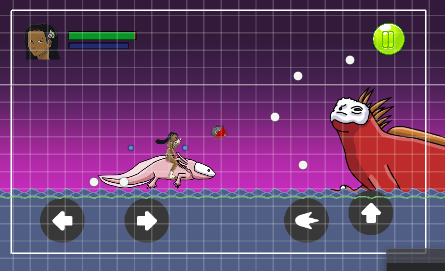
\includegraphics[width=0.6\textwidth]{05TrabajoReali/imagenes/tilemaps01.png}
    			\caption{Vista de la escena cuando se tiene un \textit{GameObject} de 
    			tipo \textit{Tilemaps} para la construcción de niveles}
    			\label{fig:TilemapPantalla}
			\end{figure}
		
		\item \textbf{\textit{Cinemachine}:} \textit{Asset} que permite controlar la 
		cámara de la escena, con este \textit{asset} se le puede indicar que objeto se 
		desea que la cámara siga y se puede asignar un área que limitara el movimiento 
		de la cámara (ver figura \ref{fig:CinemaPantalla}). \textit{Cinemachine} se 
		descarga directamente desde la tienda de \textit{assets} de \textit{Unity} y 
		fue desarrollado por los ingenieros de \textit{Unity}, lo que significa que 
		no genera conflictos o no requiere de configuraciones extras al proyecto para 
		importar. En la sección () se profundizará su funcionamiento.
			
			\begin{figure}[h]
    			\centering
    			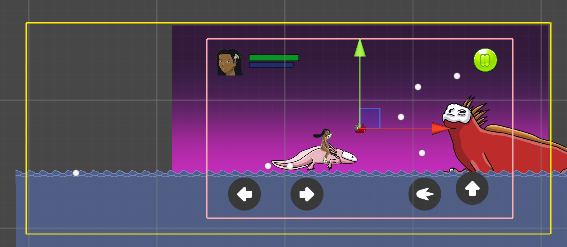
\includegraphics[width=0.6\textwidth]{05TrabajoReali/imagenes/cinemachine01.png}
    			\caption{Vista de la escena cuando se tiene un \textit{GameObject} de 
    			tipo \textit{Tilemaps} para la construcción de niveles}
    			\label{fig:CinemaPantalla}
			\end{figure}

		\item \textbf{\textit{Sprite Packer}}: Si bien no es una herramienta para 
		construcción de niveles o un \textit{asset}, esta herramienta es una de las 
		más útiles que se agregó a la nueva versión de \textit{Unity} ya que, como 
		su nombre lo indica, permite el empaquetado de \textit{sprites} (ver figura ). 
		Empaquetar 
		los \textit{sprites} es una práctica que optimiza el renderizado de objetos, 
		ya que el controlador de gráficos de \textit{Unity} realiza una sola llamada 
		por paquete cuando renderiza los objetos y con esa única llamada renderiza todos 
		los objetos de la escena que se encuentren en ese paquete; si los 
		\textit{sprites} no se encontraran dentro de un paquete el controlador de 
		gráficos de \textit{Unity} haría una llamada por cada \textit{sprite}.  
			\begin{figure}[h]
    			\centering
    			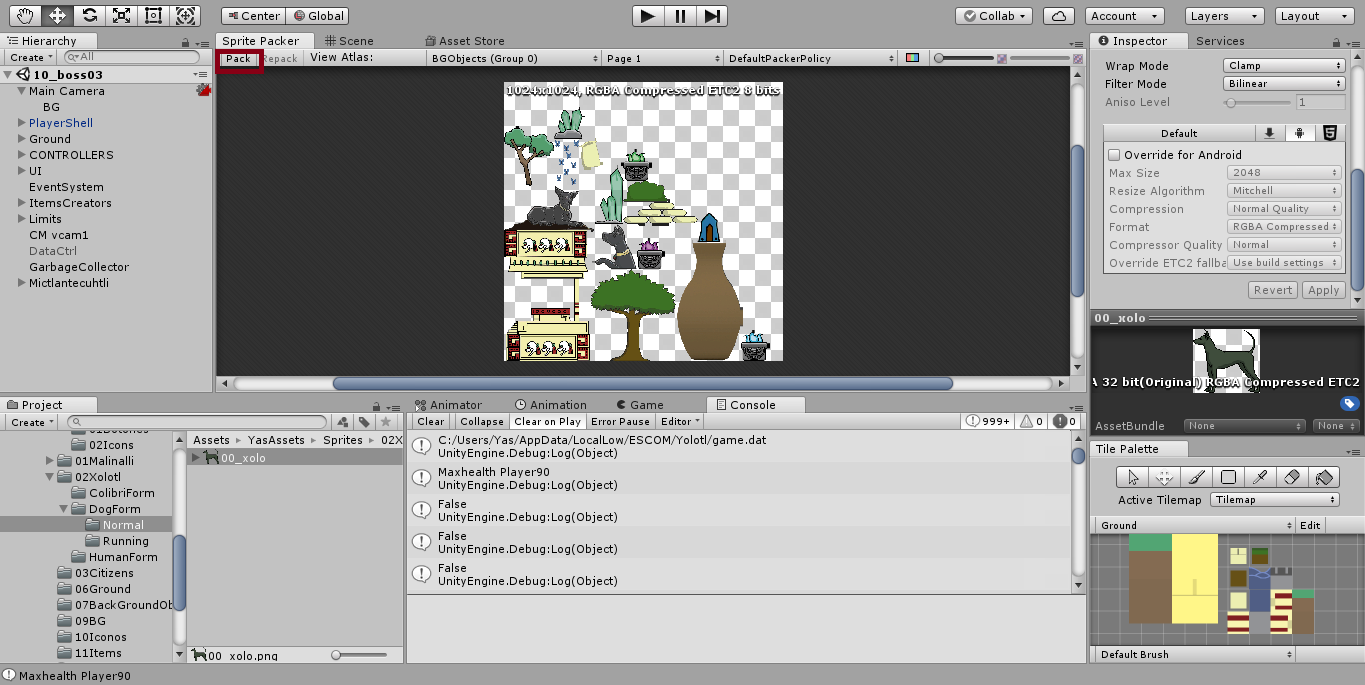
\includegraphics[width=0.6\textwidth]{05TrabajoReali/imagenes/01.png}
    			\caption{Vista de la pestaña del \textit{Sprite Packer}.}
    			\label{fig:CinemaPantalla}
			\end{figure}
	\end{itemize}
	Por el impacto que tendrían las nuevas herramientas de la versión de 
	\textit{Unity}, se propusó utilizarla en lugar de la versión 5.6.2f1. Antes 
	de actualizar la versión de \textit{Unity} se investigó si el proyecto sufriría 
	algún impacto negativo como falta de compatibilidad de componentes por la 
	diferencia de versiones. Al comprobar que existía una total compatibilidad 
	entre ambas versiones en cuanto a trasladar un proyecto de la versión 5.6.1f 
	a la versión 2017.3.1f. Se determinó que la nueva versión de \textit{Unity} 
	sería la que se emplearía para el resto del desarrollo del juego.

\subsubsection{Creación de los \textit{sprites} faltantes}
Lo siguiente a realizarse durante el sexto \textit{sprint} fueron los \textit{sprites}, 
durante las modificaciones que se definieron en Trabajo Terminal 1 fue la 
utilización de un \textit{software} de animación en dos dimensiones para generar 
los \textit{sprites} restantes; sin embargo, el cambio de \textit{software} para 
generar los sprites fue descartado, esto debido a que se adquirió una nueva 
tableta digitalizadora que agilizó la creación de \textit{sprites}. Para Trabajo 
Terminal 2 se dibujaron y digitalizaron más de 100 \textit{sprites}. Para mejorar 
la experiencia visual del jugador se animaron \textit{sprites} que en los primeros 
demos eran estáticos como es el caso de los fantasmas del segundo nivel de la 
sección de plataformas (ver figura \ref{fig:FantasmaAnimacion}). 

%%
\begin{figure}[h]
	\centering
	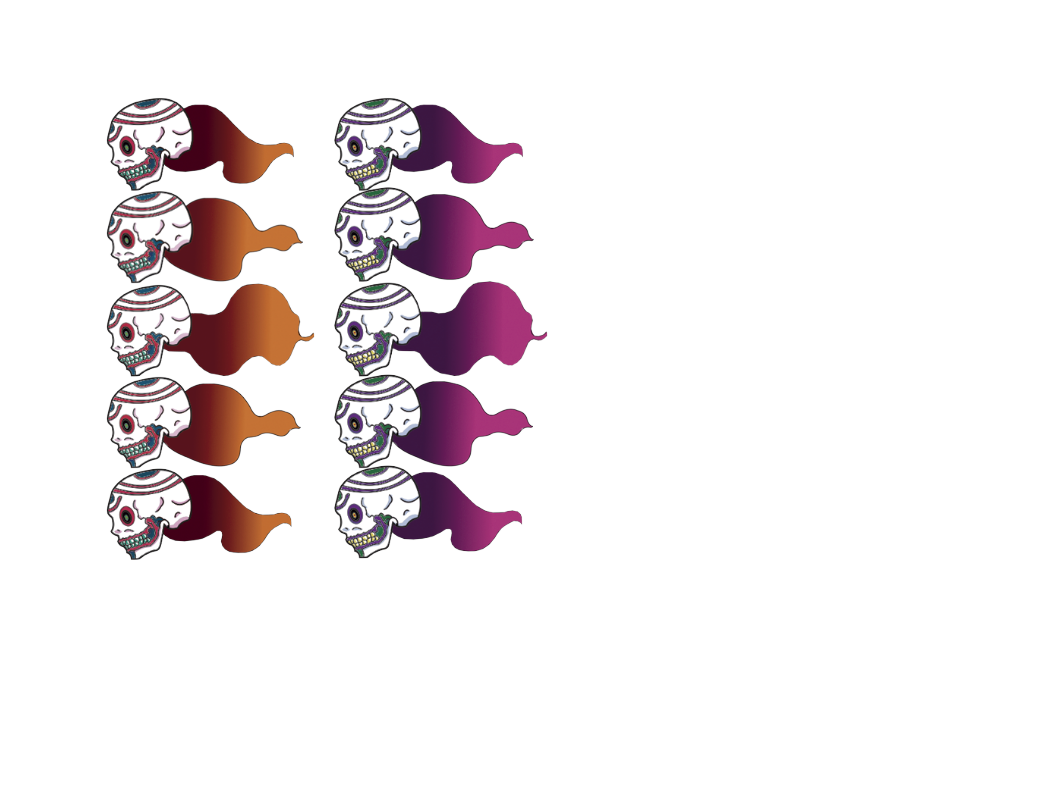
\includegraphics[width=0.4\textwidth]{05TrabajoReali/imagenes/fantasmas.png}
 	\caption{Bloques de animación para el enemigo de tipo fantasma.}
	\label{fig:FantasmaAnimacion}		
\end{figure}

Otros cambios en cuanto el aspecto visual del juego fue la integración de nuevos 
\textit{sprites} para el personaje jugable, los nuevos sprites incluyen la 
caracola que \textit{Malinalli} (ver figura \ref{fig:MalinalliCaracola}) emplea 
para atacar y que se obtiene al final del primer nivel de la sección de selva, 
estos \textit{sprites} para \textit{Malinalli} son utilizados únicamente en los 
niveles posteriores al primer nivel para darle sentido a la narrativa; para el 
segundo nivel se hizo algo parecido, los \textit{sprites} del personaje jugable 
fueron sustituidos por \textit{Malinalli} montando un ajolote (ver figura 
\ref{fig:MalinalliAjolote}), este cambio se hizo para que lo que el jugador vea 
dentro del nivel sea coherente con la narrativa propuesta y se mejore la inmersión del juego. 

\begin{figure}[h]
	\centering
	\includegraphics[width=0.4\textwidth]{05TrabajoReali/imagenes/MalinalliArma.png}
 	\caption{Bloques de animación para \textit{Malinalli} posterior a que ella obtiene la caracola.}
	\label{fig:MalinalliCaracola}		
\end{figure}

\begin{figure}[h]
	\centering
	\includegraphics[width=0.5\textwidth]{05TrabajoReali/imagenes/MalinaliAjolote.png}
 	\caption{Bloques de animación para \textit{Malinalli} montando al ajolote del segundo nivel del juego.}
	\label{fig:MalinalliAjolote}		
\end{figure}

En lo que se refiere a los Jefes de cada nivel, no solo se crearon sus respectivos \textit{sprites}, también fue necesario la creación de los \textit{sprites} referentes a sus ataques, para el caso particular de \textit{Mictlantecuhtli} se dibujaron 30 \textit{sprites} tanto para la animación del personaje como para la animación de sus respectivos ataque (ver figura \ref{fig:Mictlantecutli}). Para el diseño de la interfaz gráfica de usuario(\textit{GUI} por sus siglas en íngles) se emplearon \textit{sprites} de las paginas \textit{Kenney.nl} y \textit{Game Art 2D}. Es importante aclarar que la creación de \textit{sprites} pudo haber sido sustituida utilizando paquetes de \textit{sprites} que existen en la red y que son de licencia libre; sin embargo, con la creación de \textit{sprites} propios para el juego se consigue crearle una identidad visual propia al juego, esto permite que el jugador se identifique con mayor facilidad con el personaje y tenga una mejor asociación con el mundo y la historia que se le presenta dentro del juego [cita]. Si se desea ver a profundidad los {sprites} que se crearon se puede consultar el anexo \ref{Anexo:Personajes}. 


\begin{figure}[h]
	\centering
	\includegraphics[width=0.5\textwidth]{05TrabajoReali/imagenes/Mictlantecuhtli.png}
 	\caption{Bloques de animación para \textit{Mictlantecuhtli}, jefe final del juego.}
	\label{fig:Mictlantecutli}		
\end{figure}

\subsection{Séptimo \textit{Sprint Huddle} de Producción} 
Tal como se indicó en el sexto sprint, la siguiente tarea que se ejecutó una 
vez terminados los sprites y las maquetas de los niveles, fue la programación de 
las clases actoras. 

\subsubsection{Implementando los enemigos normales del juego} 
Las primeras clases actoras en ser programadas fueron las correspondientes a los 
enemigos normales, estas clases se programaron a la par que la clase \textit{Player}. 
Si bien la clase \textit{Player} ya estaba programada desde los primeros prototipos, 
esta clase no contaba con toda su funcionalidad implementada y la funcionalidad 
faltante tuvo que ser implementada a la par que otras clases para verificar el 
correcto funcionamiento en la interacción de clases como la de los enemigos y los 
\textit{items}.
\\
\par 
Es verdad que ya existían enemigos desde los primeros prototipos; no obstante, 
su funcionalidad tuvo que ser reimplementada a fin de ofrecer un desempeño que 
optimizará recursos y agregará nuevas funcionalidades. A continuación, se listan los 
cambios que presentan los enemigos de séptimo \textit{sprint} en relación de los 
enemigos del primer prototipo: 

	\begin{itemize}
		 \item \textbf{Áreas de acción}: En el primer prototipo los enemigos ejecutaban 
		 sus patrones de movimiento y ataque sin importar que éstos se encontraran 
		 visibles para el jugador o no. Los enemigos del séptimo \textit{sprint} 
		 cuentan con áreas de acción definida, lo que hace que sus patrones de 
		 movimientos y ataques solo se ejecuten si el jugador entra a estas áreas 
		 activas. Esto permite que el dispositivo no gaste recursos en objetos que no se 
		 encuentran visible para el jugador (ver figura ).
		 \begin{figure}[h]
    			\centering
    			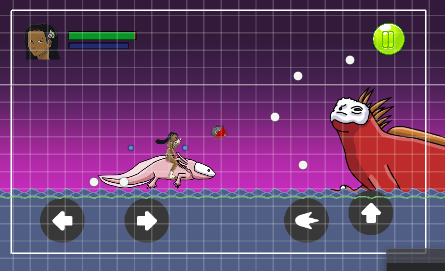
\includegraphics[width=0.6\textwidth]{05TrabajoReali/imagenes/tilemaps01.png}
    			\caption{Vista de la escena cuando se tiene un \textit{GameObject} de 
    			tipo \textit{Tilemaps} para la construcción de niveles}
    			\label{fig:EnemyArea}
			\end{figure}
		   
Cantidad de vida: En el primer prototipo todos los enemigos eran derrotados por un único disparo, esto limitaba el factor de reto del juego al no ofrecer enemigos más resistentes al ataque del jugador. En el fin de ofrecer una nueva capa de complejidad a los enemigos se agregó a la clase Enemy el atributo maxHealth y healthAmount, estos atributos serían los encargados de almacenar la máxima cantidad de vida que un enemigo puede tener y la vida actual de dicho enemigo. La cantidad de vida sólo se actualizaría cuando el enemigo fuera atacado por el jugador o cuando se reiniciara el nivel. Para la actualización de la vida del enemigo se utilizó el comando Clamp de la clase Math, este comando permite especificar rangos con valores máximos y mínimos del resultado de operaciones, esto con la finalidad de que la vida actual del enemigo nunca sea cero y nunca sobrepase a su máximo de vida.
Cantidad de daño: Al igual que con la cantidad de vida, los enemigos del primer prototipo inflingian la misma cantidad de daño sin importar su tipo; por lo que para tener enemigos más y menos fuertes se agregó el atributo damageAmount. Un enemigo puede infringir daño al jugado cada vez que toca al jugador o cuando dispara un ataque. Cada vez que un enemigo o un disparo enemigo choca con el jugador, el objeto enemigo manda a llamar el método SetHealth del Player y le envía como parámetro el valor de su atributo damageAmount, seguido de un segundo método de la clase player llamado EnemyNockBack, este método es el encargado de la animación que indica que el jugador ha recibido daño.
 Girar horizontalmente: En el primer prototipo el enemigo era incapaz de girar sus Sprite y su ataque una vez que el jugador lo sobrepasaba como se ve en la figura (). Utilizando la posición del enemigo y la posición del jugador dentro del área activa, el enemigo puede voltear si sprite y su ataque   con base al valor de la distancia entre este y el jugador: Si es menor a  1 el enemigo mantiene su orientación inicial, si es mayor a 1 el enemigo se voltea. Voltear un Sprite no representa mayor problema en código; sin embargo, el voltear un sprite cuyo colisionador no seas simétrico como el de la figura puede representar un problema cuando tiene que detectar colisiones, tal y como ocurre con los enemigos de tipo RedGost y PulpleGost; para evitar alterar la detección de colisiones se creó una nueva clase auxiliar llamada FixerCollider,  cuyo objetivo es ajustar la posición del colisionador una vez que el personaje se gira como se puede observar en la figura ().
Trigger Collider: En el primer prototipo el colisionador del enemigo tenía una configuración del tipo sólido lo que ocasionaba que cuando el enemigo chocara con otro enemigo o con algún ataque enemigo este se estancara o fuera empujado por el objeto contra el que chocaba (ver figura ). Para corregir este comportamiento se configuro el colisionador como uno de tipo trigger (ver figura ).  
Rigidbody2D: Para evitar el comportamiento mencionado en el Trigger Collider también fue necesario modificar la configuración del componente Rigidbody2D, este componente paso de estar en modo Dynamic a modo Kinematic lo que permite evitar que el objeto de juego reaccione conforme a las leyes físicas comunes.   
Para implementar cada uno de los patrones de movimiento de los enemigos fue necesario utilizar posiciones auxiliares que indicaran el límite del movimiento del personaje, salvo en la clase Vulture ya que este explota al hacer contacto con el jugador.
Para resaltar la muerte de un enemigo se agregó un efecto especial de explosión acompañado de un efecto de sonido para la explosión del personaje. Para esta funcionalidad se implementó la clase SFXCtrl y AudioCtrl para manejar los efectos de especiales y el sonido respectivamente.
	\end{itemize}

Implementando los enemigos jefes del juego.
Para la implementación de los jefes se reutilizo las configuraciones de los enemigos normales referente a componentes como Rigidbody2D y el Colisionador, el uso de la clase Enemy para el manejo de vida y el uso de los efectos de sonido y de explosiones para la muerte del jefe.
La lógica, al menos en la teoría, tras los jefes del juego fue inspirada por el jefe Roxas (ver figura ) del juego Kingdom Hearts 2 Final Mix. Dentro de Kingdom Hearts 2 Final Mix, Roxas es uno de los jefes que requiere mayor habilidad de juego para ser derrotado, ya que a diferencia del resto de los jefes del Kingdom Hearts 2 Final Mix, el patrón de ataque de Roxas era totalmente aleatorio; el jugador podía saber en qué consistía cada uno de los ataques de este jefe, pero desconocía el orden en el que estos serían ejecutados, salvo por algunos ataques que estaban condicionados a una secuencia de ataque anterior.  Con los jefes del juego Yolotl sucede algo parecido, el jugador puede llegar a conocer lo tipos de ataque que posee un jefe determinado pero la secuencia de ejecución de los ataques está programada para que sea aleatoria, lo que puede generar experiencias de juego muy sencillas o bastante retadoras para el jugador. El anterior comportamiento se logra simulando una máquina de estados con un arreglo de tipo booleano llamado whatCanDo, en el cual solo un índice puede tener el valor verdadero cada vez que se actualiza el estado y dependiendo del valor del índice del valor verdadero será el ataque que ejecutará el enemigo. Después de cada ataque el enemigo espera un tiempo determinado antes de asignar el siguiente y ejecutarlo. Para ayudar al lector a comprender el funcionamiento de los jefes se explicará nuevamente usando como ejemplo al jefe Itzpapálotl del nivel cuatro. El jefe Iztpapálotl cuenta con cuatro acciones:
waitForAction: Espera un tiempo determinado y asigna un nuevo índice valor verdadero del arreglo de valores booleanos. Se activa si whatCanDo[0] es verdadero.
shotFire: Dispara cuatro esferas de fuego que siguen al jugador y en caso de no chocar con este después de un tiempo se destruyen.  Se activa si whatCanDo[1] es verdadero.
useShell: Invoca un circulo de fuego que protege a Itzpapálotl de cualquier daño, el escudo de fuego también puede infringir daño al jugador si hace contacto con éste. Se activa si whatCanDo[2] es verdadero.
CreateButterflies: Invoca mariposas en tres puntos del campo, las mariposas también infringen daño al jugador y desaparecen después de un tiempo. Se activa si whatCanDo[3] es verdadero.
Al inicializarse el jefe Itzpapálotl whatCanDo[0] es igual a cero. Por lo que Itzpapálotl ejecuta waitForAction, al terminar la ejecución de waitForAction, whatCanDo[0] es igual a falso y un nuevo índice tiene ahora el valor verdadero. Supóngase ahora whatCanDo[2] es verdadero. Itzpapálotl ejecuta useShell, al terminar su ejecución asigna whatCanDo[2] como falso y asigna a whatCanDo[0] como verdadero. Nuevamente Itzpapálotl espera unos segundos y actualiza whatCanDo. Por la naturaleza aleatoria de la actualización, whatCanDo[2] puede ser nuevamente verdadero o lo puede ser cualquier otro índice exceptuando al 0 o a un número mayor que el índice máximo del arreglo. En la figura se muestra la verificación de los valores de whatCanDo antes de la ejecución de cualquiera de los ataques que tienen asignados. 
Por la forma en la que fue diseñado el comportamiento de la máquina de estados, el nivel de dificultad que presente el jefe esta dado en función de dos variables: damageAmount y timeBetweenAttacks, correspondientes a la cantidad de daño que el jefe puede infringir en el jugador y al tiempo que se espera para actualizar los valores de waitForAction. A mayor cantidad de daño y menor tiempo de espera entre ataques, mayor será la dificultad para derrotar al enemigo. 
Implementando los ataques enemigos del juego.
Dentro del juego existen seis tipos de ataques enemigos:
Disparos con una trayectoria definida: Este tipo de disparo sigue una trayectoria recta horizontal como se ve en la figura . Para evitar la saturación de objetos dentro del juego, todos los disparos de este tipo se destruyen después de un tiempo. Para implementar este tipo de ataque se crea un GameObject y se le agregan los siguientes componentes: 
Collisionador: El colisionador permite detectar si este ataque hace contacto con el Player o con el suelo del nivel, en el primer caso se infringe daño al player y se destruye el GameObject, en el segundo el GameObject solo se destruye. 
Rigidbody2D: El rigidbody2D se configura con la opción kinematic para evitar que el movimiento del disparo se vea afectado por la gravedad. Este componente permite en el código agregarle una velocidad al objeto.
DestryWithDelay: Componente creado por medio de la clase del mismo nombre, esta clase destruye al GameObject que la contiene después de una cantidad determinada de tiempo.
EnemyBullet: Esta clase controla en la velocidad y dirección del movimiento del disparo, también tiene como atributo el daño que causa la bala y gestiona las colisiones del objeto.
Este tipo de disparo es empleado por los enemigos de tipo RedGost, Tepeyóllotl y por Mictlantecuhtli.
Disparos que siguen al jugador: Este tipo de disparo sigue un comportamiento y configuración parecida al anterior con la diferencia que en este tipo el disparo seguirá al jugador hasta impactarse contra este o destruirse después de un tiempo si no colisiona contra el jugador.  Este comportamiento requiere que el disparo tenga una referencia a la posición del jugador para moverse hacia esta, en la figura se puede ver la implementación de disco comportamiento en código. Este ataque es utilizado por los enemigos de tipo Mictlantecuhtli, Tepeyóllotl, Itzpapálotl, Xochitonal y Tlazolteolt. Para todos estos enemigos el disparo tiene el mismo efecto que es el de infringir daño en el jugador; sin embargo, en el tipo de Tlazolteolt este tipo de disparo también puede disminuir la cantidad de Tonalli del Player.
Escudo de defensa que desaparece después de un tiempo: Este ataque es efectuado por Itzpapálotl. Al invocarse este escudo el enemigo no se ve afectado por los ataques del juador. Este escudo no puede ser destruido y desaparece después de un tiempo que se invocó. Infringe daño al jugador al hacer contacto con él.
Escudo de defensa que debe de ser destruido para desaparecer: Ataque utilizado por Tlazolteolt. Este escudo puede ser destruido por disparos del jugador y no desaparece al cabo de un tiempo. Al igual que el anterior protege al enemigo de los ataques del jugador e infringe daño si el jugador hace contacto con éste.  
Objetos que aparecen en posiciones cuya aparición tiene un tiempo de duración: Este ataque es empleado por Itzpapálotl y Mictlantecuhtli. Cuando se activa provoca que se creen instancias del GameObject que contiene la clase Butterfly. Esta clase genera un movimiento vertical ascendente e infringe daño al jugador al hacer contacto con esta. La creación de estos GameObjects se mantiene activa por un periodo de tiempo y después desactiva, ver figura .  
Objetos que aparecen en posiciones de manera periódica: Este ataque genera una lluvia de huesos o de piedras que le infringen daño al jugador una vez hacen contacto con este de lo contrario se destruyen al hacer contacto con el suelo, ver figura . Este ataque es utilizado por Mictlantecuhtli y Tepeyóllotl. 
Implementando los obstáculos.
Una de las características de un juego de plataformas es la existencia de diferentes obstáculos que el jugador debe de superar por medio de saltos. En Yolotl se diseñaron e implementaron diferentes tipos de obstáculos para ofrecer una variedad de retos al jugador, a continuación, se describe cada uno de ellos y cómo fue que fueron implementados en el juego:
Plataforma que se mueve: Es uno de los elementos más comunes de los juegos de plataforma, este   obstáculo consiste en una superficie de que se mueve de una posición a otra, ver figura . dentro del juego se creó la clase MovingPlatform para este tipo de obstáculo. MovingPlatform tiene por atributos las posiciones a las que se moverá, velocidad a la que se moverá. Para su movimiento la clase hace uso de cuatro vectores de posiciones pos01, pos02, startPos y nextPos. Pos01 y pos02 son las posiciones limite que alcanzará la plataforma, starPos es la posición hacia la que la plataforma iniciara su movimiento inicial y nextPos es la siguiente posición a la que se ira la plataforma una vez que haya alcanzado un límite. Manejar el comportamiento de las plataformas móviles con este sistema de posiciones permite que la plataforma pueda tener movimiento horizontal, vertical o diagonal. Al igual que con los enemigos las plataformas de este tipo tienen un radio de área activa para evitar que su comportamiento se ejecute si no están visibles al jugador. Asignar el movimiento de la plataforma no es suficiente para su correcto funcionamiento, ya que cuando el movimiento de la plataforma es horizontal esta se desplaza sin el personaje ya que por sí misma no es capaz de asignarle un movimiento al jugador, por tal motivo fue necesario crear una nueva etiqueta para las plataformas llamada Platform y asignar dos nuevos parámetros en las colisiones al jugador una para cuando entra en contacto con el colisionador de la plataforma y otra cuando sale. Cuando el jugador entra en contacto con el colisionador de la plataforma se le asigna un parentesco con la posición de la plataforma, lo que le permite seguir el movimiento de la plataforma, este parentesco se rompe cuando el jugador sale de la plataforma, en la figura se puede ver esto en código. Adicionalmente, se utilizó el comando OnDrawGizmos para dibujar la trayectoria de la plataforma a fin de facilitar la configuración de las plataformas móviles en la construcción de los niveles, ver figura .
Plataforma que cae: Este tipo de plataforma se cae después de que el jugador se posiciona sobre ella. Para evitar que la plataforma caiga instantáneamente una vez que el jugador ha caído sobre ella, un tiempo de retraso se le asigna a la caída.
Plataforma con más de dos posiciones de control: esta plataforma puede seguir patrones complejos movimiento como círculos, rectángulos o cudrados. Su funcionamiento es similar a la plataforma que se mueve con la diferencia de que soporta más de dos posiciones de control.
Viento: Ese obstáculo crea una corriente de viento que empuja al jugador hacia el vacío, ver figura . Para crear este obstáculo se crearon tres clases: la clase PushingObstacle, la clase WindCreator y la clase WindHelper. La primera controla el movimiento del viento a crear. La segunda crea el viento por periodos de tiempo dejando un tiempo de inactividad para que el jugador pueda pasar y la tercera activa al creador de viento cuando el jugador entra en el área activa del obstáculo, cada clase esta instanciada en un GameObject diferente. En un principio solo existían las clases PushingObstacle y WindCreator, lo que provocaba que el creador de viento creara viento aun cuando el obstáculo no era visible para el jugador lo que causaba la creación de muchos GameObjects innecesarios para el viento por lo que se creó la clase WindHelper para controlar la activación del creador de viento.  Para definir los periodos de creación de viento y de pausa de viento fue necesario probar diferentes valores para asignar los tiempos de creación y de pausa del viento. Luego de varias pruebas se definieron los siguientes tres valores 4 para el tiempo activo de creación, 8 para el tiempo de pausa de viento y 0.4 para la pausa entre creación de instancias de viento.
Estalagmitas: Este obstáculo se cae e infringe daño en el jugador cuando éste pasa por debajo del obstáculo, ver figura .  Para implementar este obstáculo se crearon dos clases: Stalagmite y StalagmiteCtrl. La primera clase gestiona la caída del objeto y el daño que le infringe al jugador si choca con este o la destrucción del objeto en caso de que choque con el suelo. La segunda clase se encarga de indicarle a la clase Stalagmite que el jugador va a pasar bajo de ella para que inicie su caída.  En la figura se puede ver la configuración de ambos objetos dentro de un nivel.
Obstáculo que hace daño: este obstáculo infringe daño al jugador cuando éste hace contacto con él y no puede ser destruido por el mismo. Este tipo de obstáculo se puede encontrar en el segundo nivel en la etapa de plataforma. Para su implementación se creó la clase DamageObstacle y esta gestiona el daño que infringe el obstáculo pudiendo generar obstáculos que causen más o menos daños que otros.
Xólotl en su forma Colibrí: Este obstáculo tiene un comportamiento parecido a la plataforma con más de dos posiciones de control anteriormente descrita, con la diferencia de que su movimiento describe una línea y no un circuito cerrado y que al morir el jugador este obstáculo regresa a su posición inicial. Este obstáculo aparece únicamente en el nivel 6, donde el jugador deberá cruzar distintos segmentos del mapa sobre este obstáculo y tendrá que vencer a los enemigos que vayan apareciendo para avanzar.

 Implementando los ítems, los objetos coleccionables y los puntos de guardado.
Las ultimas clases actoras en ser implementadas fueron los ítems, los objetos coleccionables y los puntos de guardado, ya que en el caso de los ítems y los checkpoins se necesitaba que el jugador sufriera daño, gastara tonalli o muriera ya fuera a causa de enemigos u obstáculos. 
Dentro del juego existen dos tipos de Items: Los que recuperan cantidad de vida y los que recuperan cantidad de tonalli. Ambos tienen un funcionamiento similar: como atributos sus respectivas clases tienen una cantidad de lo que van a restaurar (sea tonalli o vitalidad), al hacer contacto con el jugador le incrementan dicho atributo en la cantidad que tienen asignada y se destruyen mostrando un efecto de brillos y un efecto de sonido. 
En lo que se refiere a los objetos coleccionables dentro del juego se creo la clase CollectableObjects encargada de destruir los objetos coleccionables una vez que el jugador los tocaba, dejando la parte de actualizar el marcador al jugador. Para poder lograr la actualización del atributo score del jugador se asignaron etiquetas para los objetos collecionables y dependiendo de dichas etiquetas se gestiona la actualización de los marcadores, esto debido la función de los objetos coleccionables depende directamente del nivel, por ejemplo para los perros que aparecen en el segundo nivel, hacer contacto con uno de ellos no solo actualiza el marcador sino también incrementa el poder que tendrá el Jefe de este nivel, por lo que gráficamente la actualización visual del marcador deberá incluir cuantos perros se han tocado y en cuanto se ha incrementado el poder del jefe(ver figura ); mientras que en el nivel 4, los coleccionables son llaves y su función son la de desbloquear la transición al siguiente nivel solo si se han juntado todas las llaves; visualmente esta actualización solo requiere de la actualización de un elemento en pantalla (ver figura ). Para solucionar esto se crearon dos etiquetas para cada tipo de coleccionable: CollectableDog y CollectableKey.  Dejando al gestor de colisiones de la clase Player verificar por medio de la etiqueta de qué tipo de coleccionable se trata e invoca al controlador de la interfaz gráfica de los marcadores del juego o HUB, ver figura .
	\chapter{Resultados obtenidos}

	\chapter{Conclusiones}


	
	%===== Bibliografia
	\bibliographystyle{IEEEtran}
	\bibliography{00Biblio/02ProblemaA.bib,00Biblio/03MarcoMotor.bib,00Biblio/03MarcoTeoCultura.bib,00Biblio/03MarcoTeoDesarrolo.bib,00Biblio/03MarcoTeoVideo.bib}
	%\bibliography{03MarcoTeoVideo.bib, 03MarcoTeoCultura.bib}%, 00Biblio/03MarcoMotor.bib, 00Biblio/03MarcoTeoCultura.bib 00Biblio/03MarcoTeoDesarrolo.bib,
	%%\bibliography{00Biblio/05TrabRealizado.bib}
	
	\chapter{Anexos}
En este capitulo se encuentran todos los anexos que se mencionaron en los 
capitulos anteriores.

\section{Interfaces}\label{Anexo:Intefaces}

\begin{figure}[h]
    \centering
    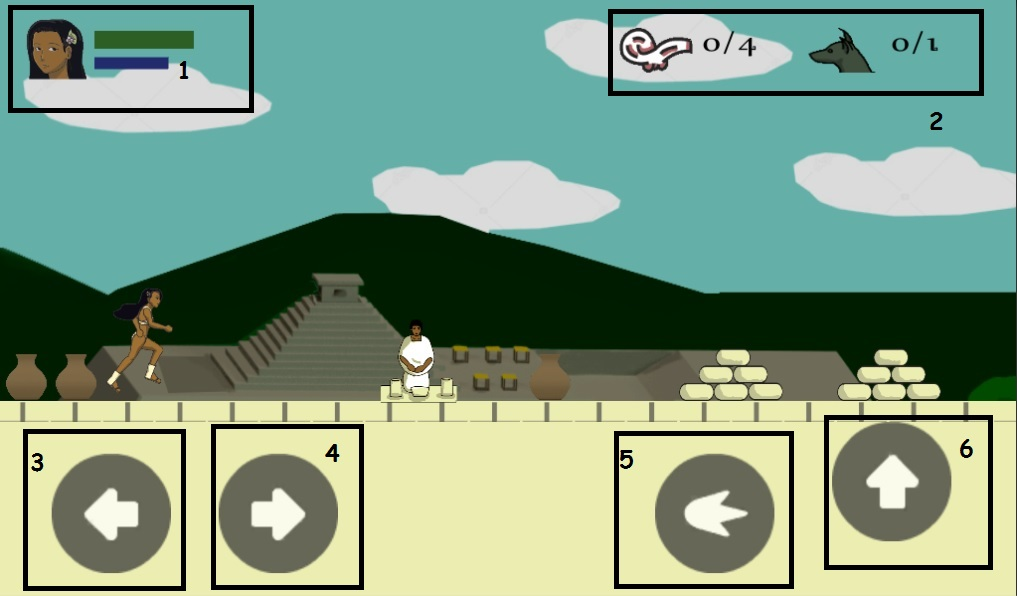
\includegraphics[width=0.25\textwidth]{Anexos/Interfaces/ControlCorrerDer.jpg}
    \caption{a nice plot}
    \label{fig:mesh1}
\end{figure}
\section{Diseño de Personajes} \label{Anexo:Personajes}

%	====	Malinalli	====
\begin{figure}[h]
  		\centering
   		\subfigure[Sprites Malinalli para el primer nivel.] {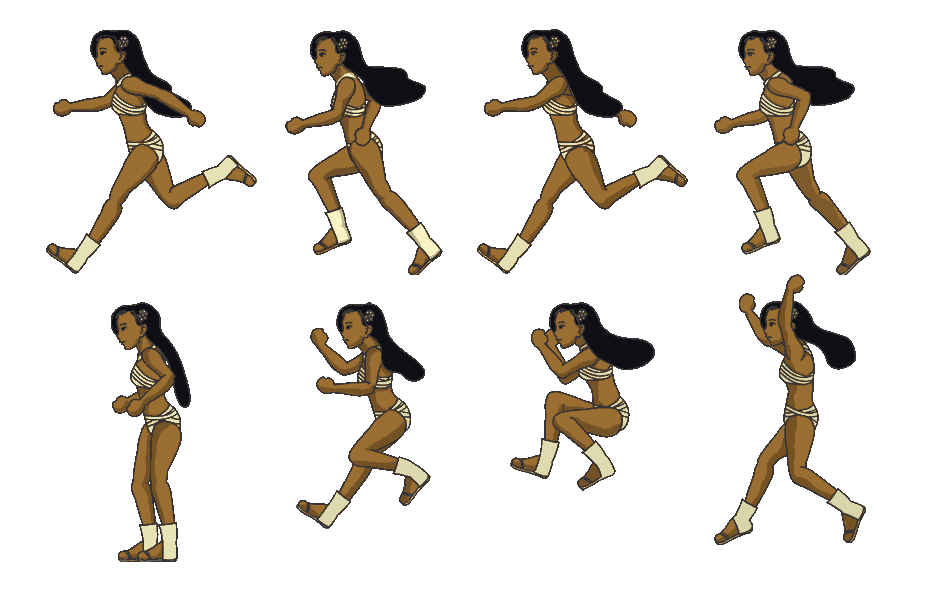
\includegraphics[width=0.3 \textwidth]{Anexos/disenios/MalinalliNormal.png}}
   
 		\subfigure[Sprites Malinalli de nado para el segundo nivel.]{\includegraphics[width=0.3 \textwidth]{Anexos/disenios/MalinaliAjolote.png}}
 	
		\subfigure[Sprites Malinalli de salto para el segundo nivel.] {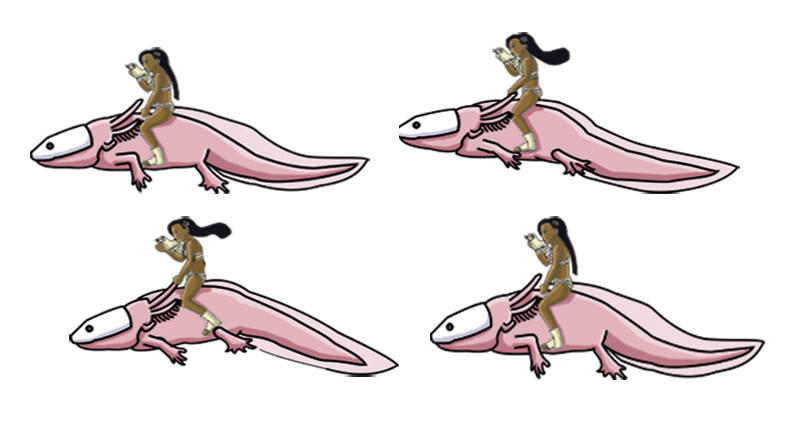
\includegraphics[width=0.3 \textwidth]{Anexos/disenios/MalinaliAjolotesalto.png}}
		
		\subfigure[Sprites Malinalli para los niveles posteriores al segundo nivel.] {\includegraphics[width=0.3 \textwidth]{Anexos/disenios/MalinalliArma.png}}
		
  		\caption{Sprites del personaje jugable (Autoria propia)}
  		\label{fig:Malinalli}
\end{figure} 

%	====	Xolotl	====
\begin{figure}[h]
    \centering
    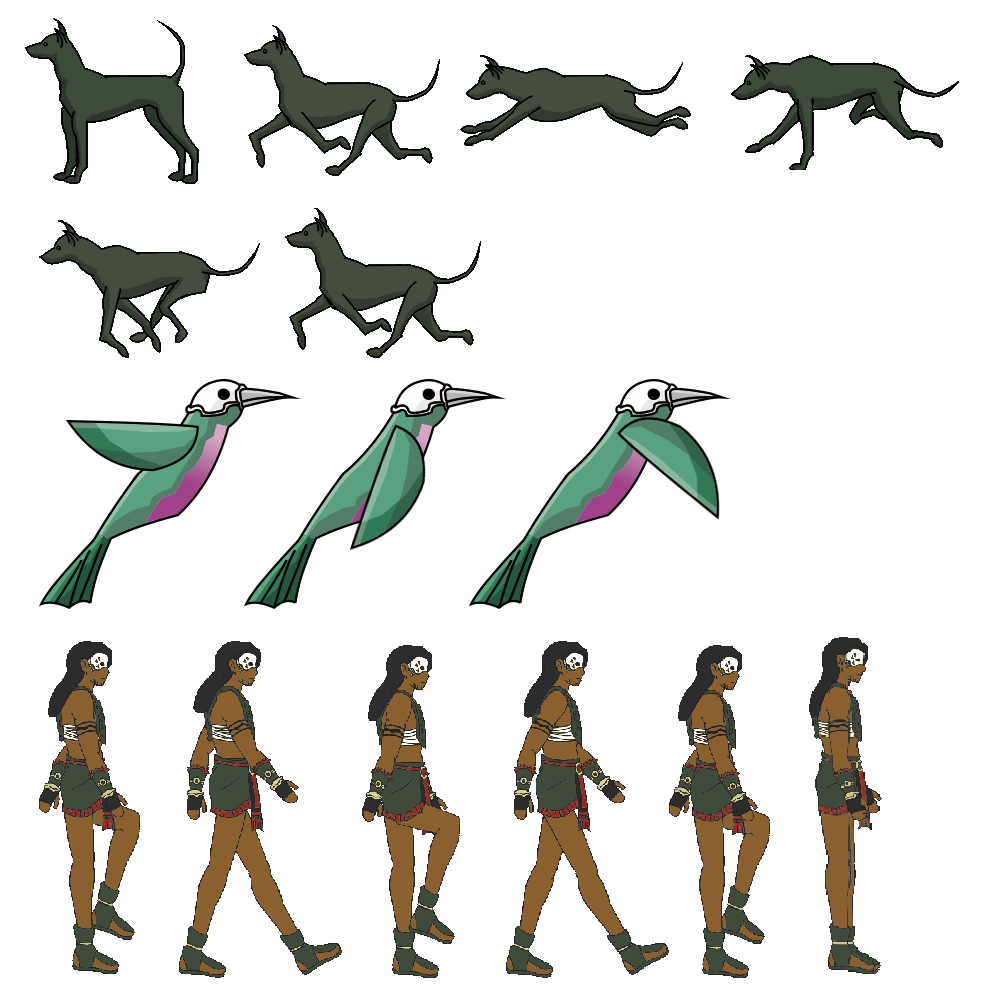
\includegraphics[width=0.40\textwidth]{Anexos/disenios/Xolotl.png}
    \caption{Sprites para las diferentes formas que toma Xólotl a lo largo del juego.}
    \label{fig:Xolotl}
\end{figure}

%	====	Enemigos normales	====
\begin{figure}[h]
    \centering
    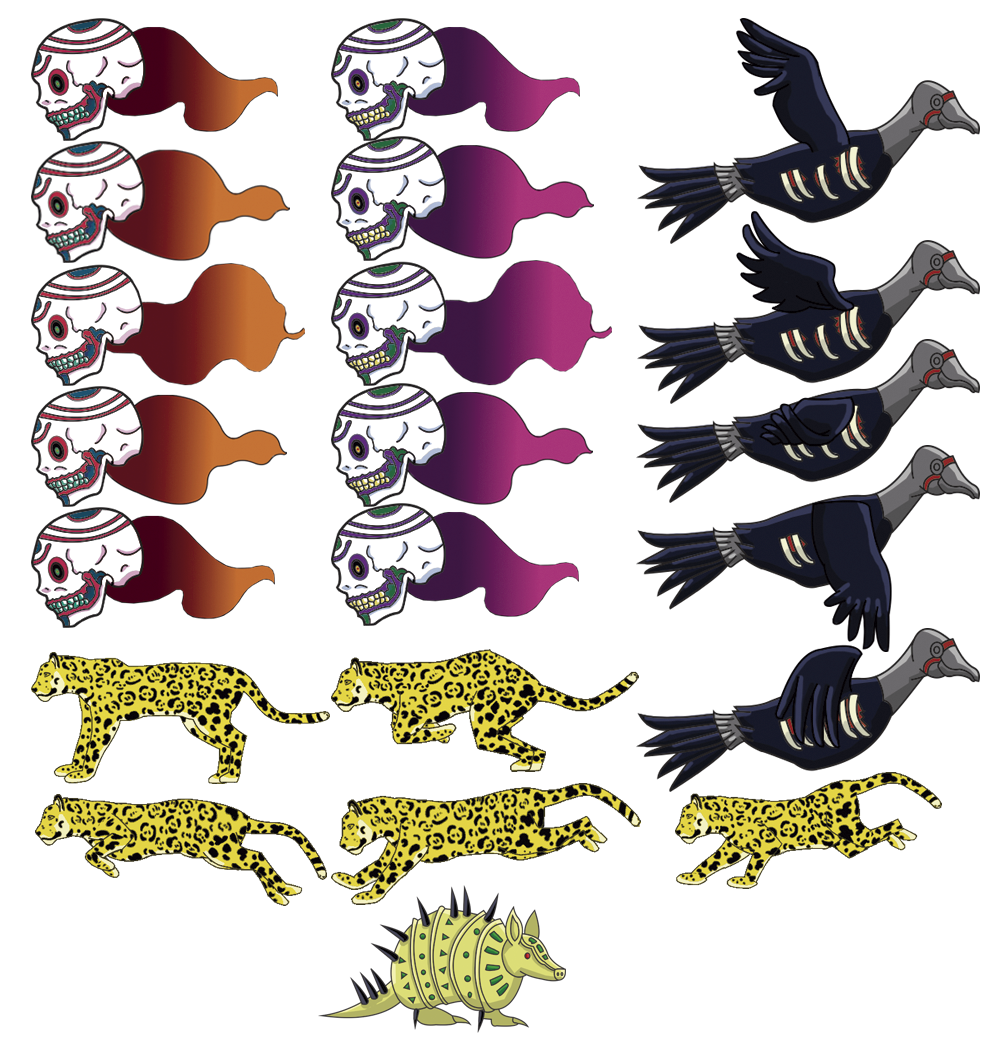
\includegraphics[width=0.40\textwidth]{Anexos/disenios/EnemigosNormales.png}
    \caption{Sprites para los enemigos normales del juego.}
    \label{fig:NorlmalEnemy}
\end{figure}

%	====	Jefes	====
\begin{figure}[h]
    \centering
    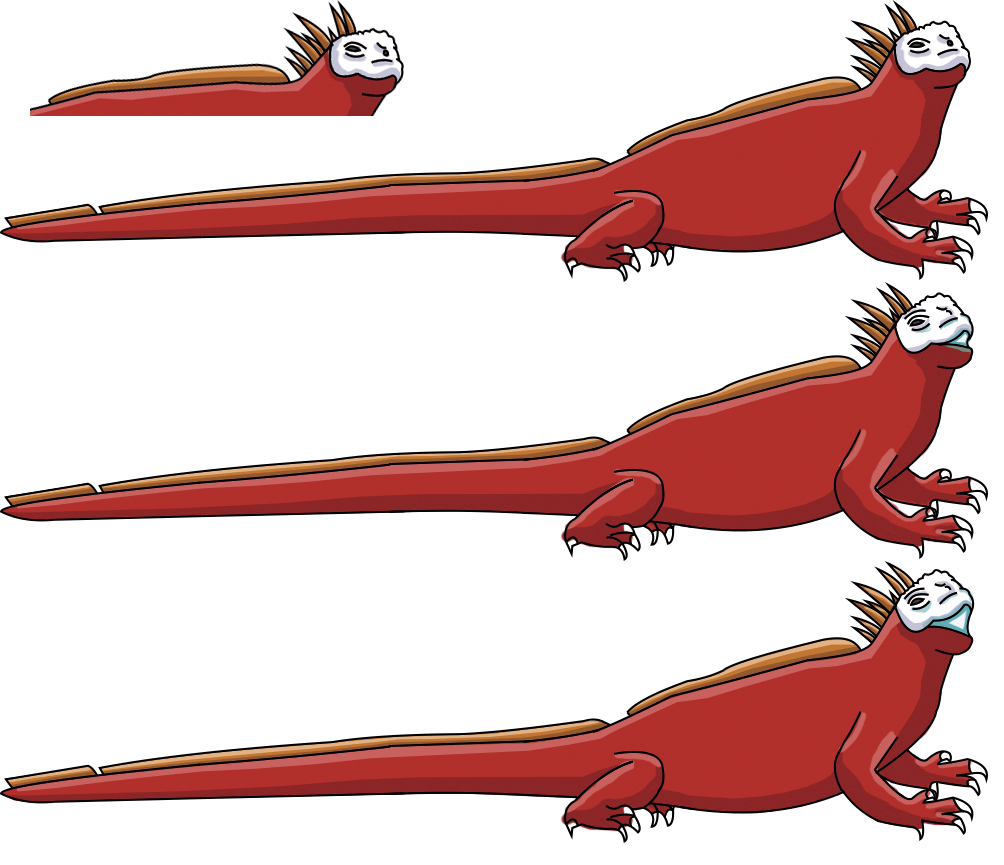
\includegraphics[width=0.40\textwidth]{Anexos/disenios/Xochitonal.png}
    \caption{Sprites de Xochitonal.}
    \label{fig:Xochitonal}
\end{figure}

\begin{figure}[h]
    \centering
    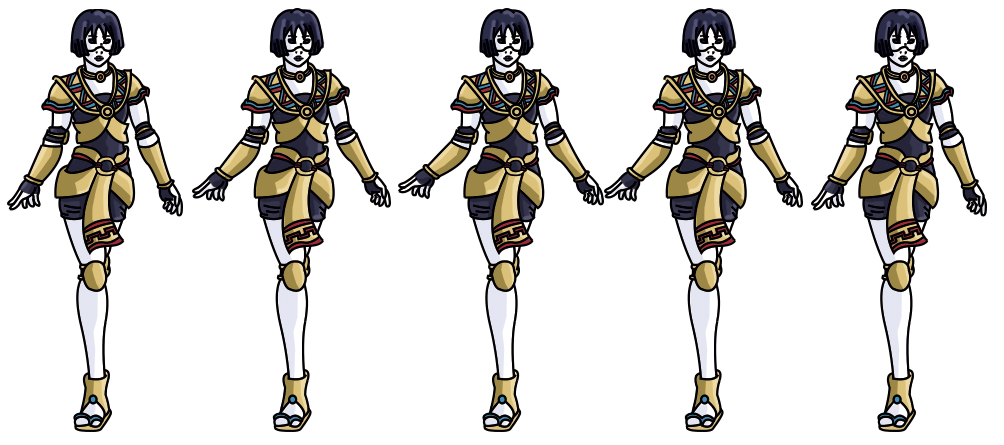
\includegraphics[width=0.40\textwidth]{Anexos/disenios/Itzpapalotl.png}
    \caption{Sprites de Itzpapálotl.}
    \label{fig:Itzpapalotl}
\end{figure}

\begin{figure}[h]
    \centering
    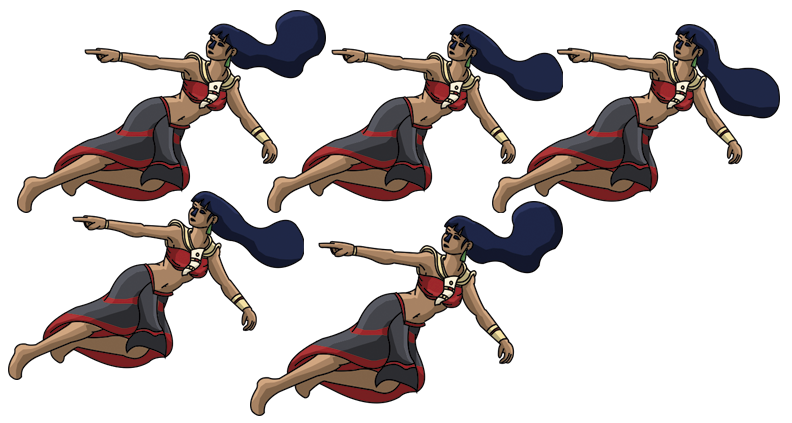
\includegraphics[width=0.40\textwidth]{Anexos/disenios/Tlazolteotl.png}
    \caption{Sprites de Tlazolteotl.}
    \label{fig:Tlazolteotl}
\end{figure}

\begin{figure}[h]
    \centering
    
\includegraphics[width=0.50\textwidth]{Anexos/disenios/Tepeyollotl.png}
    \caption{Sprites de Tepeyollotl.}
    \label{fig:Tepeyollotl}
\end{figure}

\begin{figure}[h]
    \centering
    \includegraphics[width=0.50\textwidth]{Anexos/disenios/Mictlantecuhtli.png}
    \caption{Sprites de Mictlantecuhtli.}
    \label{fig:Mictlantecuhtli}
\end{figure}

%	====	Ataques Enemigos	====
\begin{figure}[h]
    \centering
    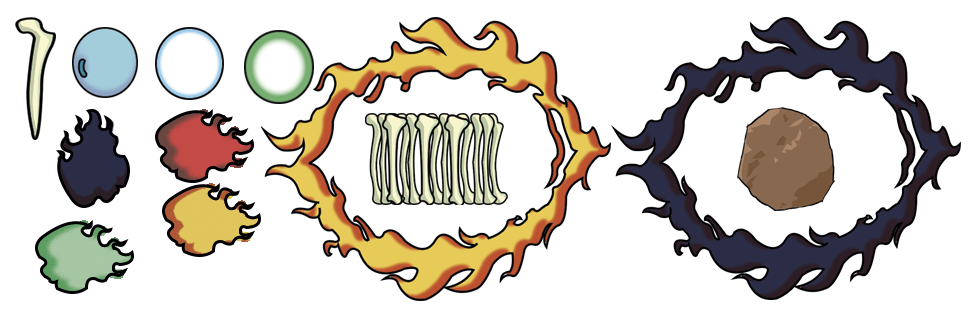
\includegraphics[width=0.50\textwidth]{Anexos/disenios/Ataques.png}
    \caption{Sprites de los ataques de los personajes.}
    \label{fig:Mictlantecuhtli}
\end{figure}

	
\end{document}